\chapter{Learned Template Retrieval}
\label{chapter:template}

%\chapres{\lipsum[1]}{\lipsum[2]}
\chaptoc



\section{Automatic template retrieval: a dual challenge}

Talk about why is important to optimize this process, focusing 
here only on the retrieval of templates, not the whole generation and
pipeline presented before

Define formally the problem, which requires to obtain a single or a set of templates 
that follow the web article content/requirements, and also that are both not 
so similar between them and also follow's historical usage (popularity).

To check if they are similar between them, it requires to understand, model and create a 
similarity metric of templates based on their internal organization (topology)

This task can be solved in two different contexts:

\begin{enumerate}
    \item Retrieve templates  in an isolated setup, i.e. a single template for a single article, following the requirements above.
    This works as a retrieval system to assist the selection of templates, in a stage where no full page is planned yet, or as a isolated
    module to deploy in \melody.

    \item Retrieve templates, but this time in a global page-aware context,
     where the choice of one article impacts the other articles in the same page. 
     This is the context where our page generation method  and the web to print pipeline 
     works.
\end{enumerate}

\section{Template similarity modelling}
\label{section:modelling-similarity}

Both the single-article retrieval setting and the page-aware scoring setting require comparing the internal topological structure of two templates $\templateobj{1}$ and $\templateobj{2}$, in order to assess how structurally similar or distinct their zonings are. In this context, standard metrics such as Intersection-over-Union (IoU) or Jaccard index (\secref{sec:sota-geometric-similarity}) are insufficient: they are sensitive to small misalignments, and in cases with no overlap they provide zero gradients, making optimization difficult~\cite{patil_layoutgmn_2021}. 

Two complementary similarity measures are proposed to address this:
\begin{itemize}
    \item \textbf{Template- and distance-based Intersection over Union}, an analytical, distance-IoU~\cite{zheng_distance-iou_2019} based measure that is fast to compute and requires no training data. Being analytical, however, it remains IoU-based, and therefore the misalignment issues described above can still persist.
    \item \textbf{Template-based Graph Matching Network}, a learned measure that captures richer topological relationships considering inner blocks and their classes. Because it requires training data, the former similarity measure is used to weakly label the triplets on which it is trained.
\end{itemize}
Both measures are presented in turn below, and are later compared empirically and qualitatively.

\subsection{Similarity measure 1: Template- and distance-based Intersection over Union ($\tdiou{\cdot}{\cdot}$)}

This first similarity measure is an analytical, geometry-based metric that provides a first approximation to layout similarity, without requiring any training data.

This similarity metric, coined Template- and distance-based Intersection over Union ($\tdiou{\cdot}{\cdot}$), which adapts the Distance-IoU loss~\cite{zheng_distance-iou_2019} to multi-element layouts, considers both the overlap between regions and the distance between their centers, providing a continuous measure of geometric alignment.

The computation of $\tdiou{\cdot}{\cdot}$ involves three steps: rescaling templates for fair comparison, matching elements of the same class, and summing the similarity of matched elements. Formally, for templates $\templateobj{1}$ and $\templateobj{2}$:
\begin{equation}
\tdiou{\templateobj{1}}{\templateobj{2}} = C_S \, C_M \, \frac{\sum_{(\zblock{1}{j},\zblockrescaled{2}{k}) \in M} \diouplusone{\zblock{1}{j}}{\zblockrescaled{2}{k}}}{|M|},
\label{eq:tdiou}
\end{equation}


where $\zblockrescaled{2}{k}$ are elements of $\tilde{\templateobj{2}}$, which corresponds to $\templateobj{2}$ rescaled to match $\templateobj{1}$ ($\Htemp{\tilde{\templateobj{2}}} = \Htemp{\templateobj{1}} $, $\Wtemp{\tilde{\templateobj{2}}} = \Wtemp{\templateobj{1}}$), $M$ is the set of matched element pairs, $C_S$ penalizes dimensional differences, and $C_M$ accounts for unmatched elements. The rest of this section gives more details about the different terms and notions introduced here.  

%TODO: Image about this

\subsubsection*{Similarity measure (\diouplusone{\templateobj{1}}{\templateobj{2}})}
\label{sec:tdiou:diouplusone}


Starting from a reimplementation using CGAL~\cite{cgal} of \diou{\templateobj{1}}{\templateobj{2}}~\cite{zheng_distance-iou_2019} in $[-1,1]$, \diouplusone{\templateobj{1}}{\templateobj{2}} is defined as:
\[
\diouplusone{\templateobj{1}}{\templateobj{2}} = \diou{\templateobj{1}}{\templateobj{2}} + 1,
\]
ensuring non-negative values. 

CGAL~\cite{cgal} was adopted for this reimplementation because template blocks may be arbitrary convex or concave polygons, possibly with holes, rather than simple axis-aligned rectangles. CGAL provides robust and fast C++ implementations of the polygon intersection and union operations this requires.
\subsubsection*{Rescaling and dimensional penalty}
\label{sec:tdiou:rescaling}

Templates are rescaled for element-wise comparison. Let $\tilde{\templateobj{2}}$ denote $\templateobj{2}$ rescaled to match $\templateobj{1}$. The penalty factor $C_S$ reduces similarity when $\templateobj{2}$ differs substantially from $\templateobj{1}$ in area, aspect ratio, or orientation:
\begin{align*} 
    C_S =& f_{\sigma_{1},\gamma_1}(\Htemp{\templateobj{1}}\Wtemp{\templateobj{1}} - \Htemp{\templateobj{2}}\Wtemp{\templateobj{2}}) \,
           f_{\sigma_2,\gamma_2}(\arctan(\Htemp{\templateobj{1}}/\Wtemp{\templateobj{1}}) - \arctan(\Htemp{\templateobj{2}}/\Wtemp{\templateobj{2}})) \nonumber\\
         & \, g_{\sigma_3,\gamma_3}((\arctan(\Htemp{\templateobj{1}}/\Wtemp{\templateobj{1}}) - \pi/4)(\arctan(\Htemp{\templateobj{2}}/\Wtemp{\templateobj{2}}) - \pi/4)),
\end{align*}
with
\[
f_{\sigma,\gamma}(t) = \exp\left(-\frac{(t/\gamma)^2}{2\sigma^2}\right), \quad
g_{\sigma,\gamma}(t) =
\begin{cases}
\exp\left(\frac{t/\gamma}{\sigma}\right), & t < 0,\\
1, & t \ge 0.
\end{cases}
\]

Each of the three factors composing $C_S$ targets a distinct source of dimensional mismatch:
\begin{itemize}
    \item the first factor, $f_{\sigma_1,\gamma_1}$, penalizes differences in total area between $\templateobj{1}$ and $\templateobj{2}$;
    \item the second factor, $f_{\sigma_2,\gamma_2}$, penalizes differences in aspect ratio between the two templates;
    \item the third factor, $g_{\sigma_3,\gamma_3}$, further penalizes the case where $\templateobj{1}$ and $\templateobj{2}$ fall on opposite sides of a square aspect ratio (e.g., one portrait-oriented and the other landscape-oriented), since such an orientation flip is perceptually more disruptive than a comparable difference in aspect ratio alone.
\end{itemize}
Both $f_{\sigma,\gamma}$ and $g_{\sigma,\gamma}$ decay smoothly toward zero as their argument grows in magnitude, so $C_S$ approaches zero, and the overall similarity \tdiou{\templateobj{1}}{\templateobj{2}} collapses accordingly, increasing the difference between $\templateobj{1}$ and $\templateobj{2}$.

\subsubsection*{Element matching and penalty}
\label{sec:tdiou:matching}
Elements $\zblock{1}{j} \in \templateobj{1}$ and $\zblockrescaled{2}{k} \in \tilde{\templateobj{2}}$ are matched based on $\diouplusone{\templateobj{1}}{\templateobj{2}}$ similarity and class correspondence, formulated as an assignment problem solvable with the Hungarian algorithm~\cite{hungarian}. The set of matched pairs is $M$. Unmatched elements are penalized via:
\[
C_M = \frac{1}{2 \, \Htemp{\templateobj{1}}\Wtemp{\templateobj{1}}} \sum_{(\zblock{1}{j},\zblockrescaled{2}{k}) \in M} \big( area(\zblock{1}{j} + area(\zblockrescaled{2}{k}) \big).
\]
This ensures \tdiou{\templateobj{1}}{\templateobj{2}} accounts for both matched element quality and structural differences.
%TODO figure for matching

\subsection{Similarity measure 2: Template-based Graph Matching Network ($\gmn{\cdot}{\cdot}$)}

This second similarity measure is a learned measure that captures richer topological relationships considering inner blocks and their classes, as a way to prevent the misalignment issues of IoU-based measures.

The proposed method is a Graph Matching Network (GMN) architecture~\cite{patil_layoutgmn_2021}, here referred to as \gmnNetwork, was implemented and retrained for the purpose of this work, following the cross-graph attention mechanism and triplet-based training scheme described in \secref{sec:sota-gmn}. Templates are represented as directed, fully connected graphs over their constituent elements, in the same manner as LayoutGMN, and \gmnNetwork is trained on triplets built from $\tdiou{\cdot}{\cdot}$ thresholds rather than plain Intersection-over-Union. Consequently, \gmnNetwork produces a similarity function, denoted $\gmn{\cdot}{\cdot}$, that can be applied to any pair of templates $\templateobj{1}$ and $\templateobj{2}$. Following the sign convention of the LayoutGMN implementation, this raw score is negative by construction and satisfies $\gmn{\templateobj{1}}{\templateobj{2}} = 0$ if the templates are identical, growing more negative as their structures diverge.

The use of the $\gmn{\cdot}{\cdot}$ metric varies depending on the application; in single-article context (\secref{section:template-retrieval-single-article}), the absolute value of this metric is used to define the distance for clustering and retrieval. In the page-aware setting of \neuralmethod\ (\secref{sec:gwes-gmn-mapping}), the same score is instead mapped into a bounded $[0,1]$ affinity through a Gaussian kernel, since that context requires a normalized similarity matrix rather than an unbounded distance.


\subsection{Empirical comparison}

\subsubsection*{Motivation}

To assess which similarity measure better reflects human perception, an online study was conducted. Each trial consisted of: (1) a reference template $\templateobj{R}$ shown for 2 seconds, followed by (2) a selection scene where participants chose the template most similar to $\templateobj{R}$ between two options $\templateobj{O_1}$ and $\templateobj{O_2}$. This design specifically targets immediate perceptual judgment rather than deliberate analysis, since participants are given only a few seconds to decide.

\subsubsection*{Research questions and hypothesis}

This study tests whether $\tdiou{\cdot}{\cdot}$ or $\gmn{\cdot}{\cdot}$ better aligns with immediate human judgments of layout similarity.

\subsubsection*{Experimental design}

\paragraph{Clustering using both methods}

Using the distance $d(\cdot,\cdot)$ defined by:
\begin{equation}
d_{tdIoU}(\templateobj{1},\templateobj{2}) = |\tdiou{\templateobj{1}}{\templateobj{2}}|,
\label{eq:clustering-distance-definition}
\end{equation}
templates are organized via agglomerative clustering with a threshold $\tdiouclusterthreshold$. Starting from singleton clusters, pairs of clusters are merged when their average inter-template distance is below $\tdiouclusterthreshold$. This produces a set of clusters $\tdiouclusters$.

At the same time, a set of clusters $\gmnclusters$ can be generated using an analog distance $d_{GMN}(\templateobj{1},\templateobj{2}) = |\gmn{\templateobj{1}}{\templateobj{2}}|$, and the corresponding inter-template maximum average distance of $\gmnclusterthreshold$.

Note that both $\tdiouclusterthreshold$ and $\gmnclusterthreshold$ were set to produce a reasonable, but also equivalent and comparable number of clusters between the methods. Specifically, $\tdiouclusterthreshold = 1.1$ and $\gmnclusterthreshold=2.8$, producing $|\tdiouclusters| = 80$ and $|\gmnclusters| = 81$ respectively, with a similar distribution.

\paragraph{Triplet definition}
Each trial involved a triplet $(R,O_1,O_2)$. $\templateobj{O_1}$ was chosen as a neighbor of $\templateobj{R}$ according to \tdiou{\templateobj{R}}{\templateobj{O_1}} but not \gmn{\templateobj{R}}{\templateobj{O_1}}, and $O_2$ as a neighbor according to \gmn{\templateobj{R}}{\templateobj{O_2}} but not \tdiou{\templateobj{R}}{\templateobj{O_2}}.  40 randomnly-selected triplets were generated this rule (examples in \figref{fig:online_experiment}(b)).

\paragraph{Experimental protocol}
Participants completed a short questionnaire on reading habits, followed by four blocks of 40 trials each, and a post-experiment questionnaire on their experience. Responses were collected via \emph{Labvanced}~\cite{labvanced}, yielding $42 \times 4$ votes per triplet.

\subsubsection*{Population}

The study recruited $42$ anonymous participants via \emph{Prolific}~\cite{prolific}.

\subsubsection*{Results}
Across all trials and participants, votes were evenly split between $O_1$ and $O_2$, resulting in a global 50:50 ratio between both methods. This indicates that neither similarity measure dominates when results are aggregated.

However, a finer-grained analysis at the triplet level reveals a more structured pattern. \figref{fig:online_experiment}(a) shows the percentage of $O_2$ (GMN) selections for each triplet, along with the interquartile range defined by Q1 and Q3 (25\%--75\% of responses). Only six triplets ($15\%$) fall (in average) within the 40\%--60\% range, indicating near-indifference between the two measures. In contrast, most triplets exhibit a clear preference, as reflected by asymmetric interquartile ranges.

Focusing on the interquartile interval, $45\%$ of the triplets (triplets $\{23,\dots,40\}$) show a majority preference for $\gmn{\cdot}{\cdot}$, while $40\%$ of the triplets (triplets $\{1,\dots,15\}$) favor $\tdiou{\cdot}{\cdot}$. This suggests that participant judgments are highly dependent on the specific structural and geometric characteristics of the templates involved.

To better understand these differences, two representative triplets (10 and 35) are illustrated in \figref{fig:online_experiment}(b). In triplet 10, participants predominantly selected $O_1$, consistent with the high geometric overlap captured by $\tdiou{\cdot}{\cdot}$, despite differences in the presence of small layout elements. Conversely, in triplet 35, participants favored $O_2$, where $\gmn{\cdot}{\cdot}$ captures higher structural similarity, while $\tdiou{\cdot}{\cdot}$ is more strongly influenced by variations in the size of dominant elements such as the main image and body text.


\begin{figure}[thbp]
    \centering
    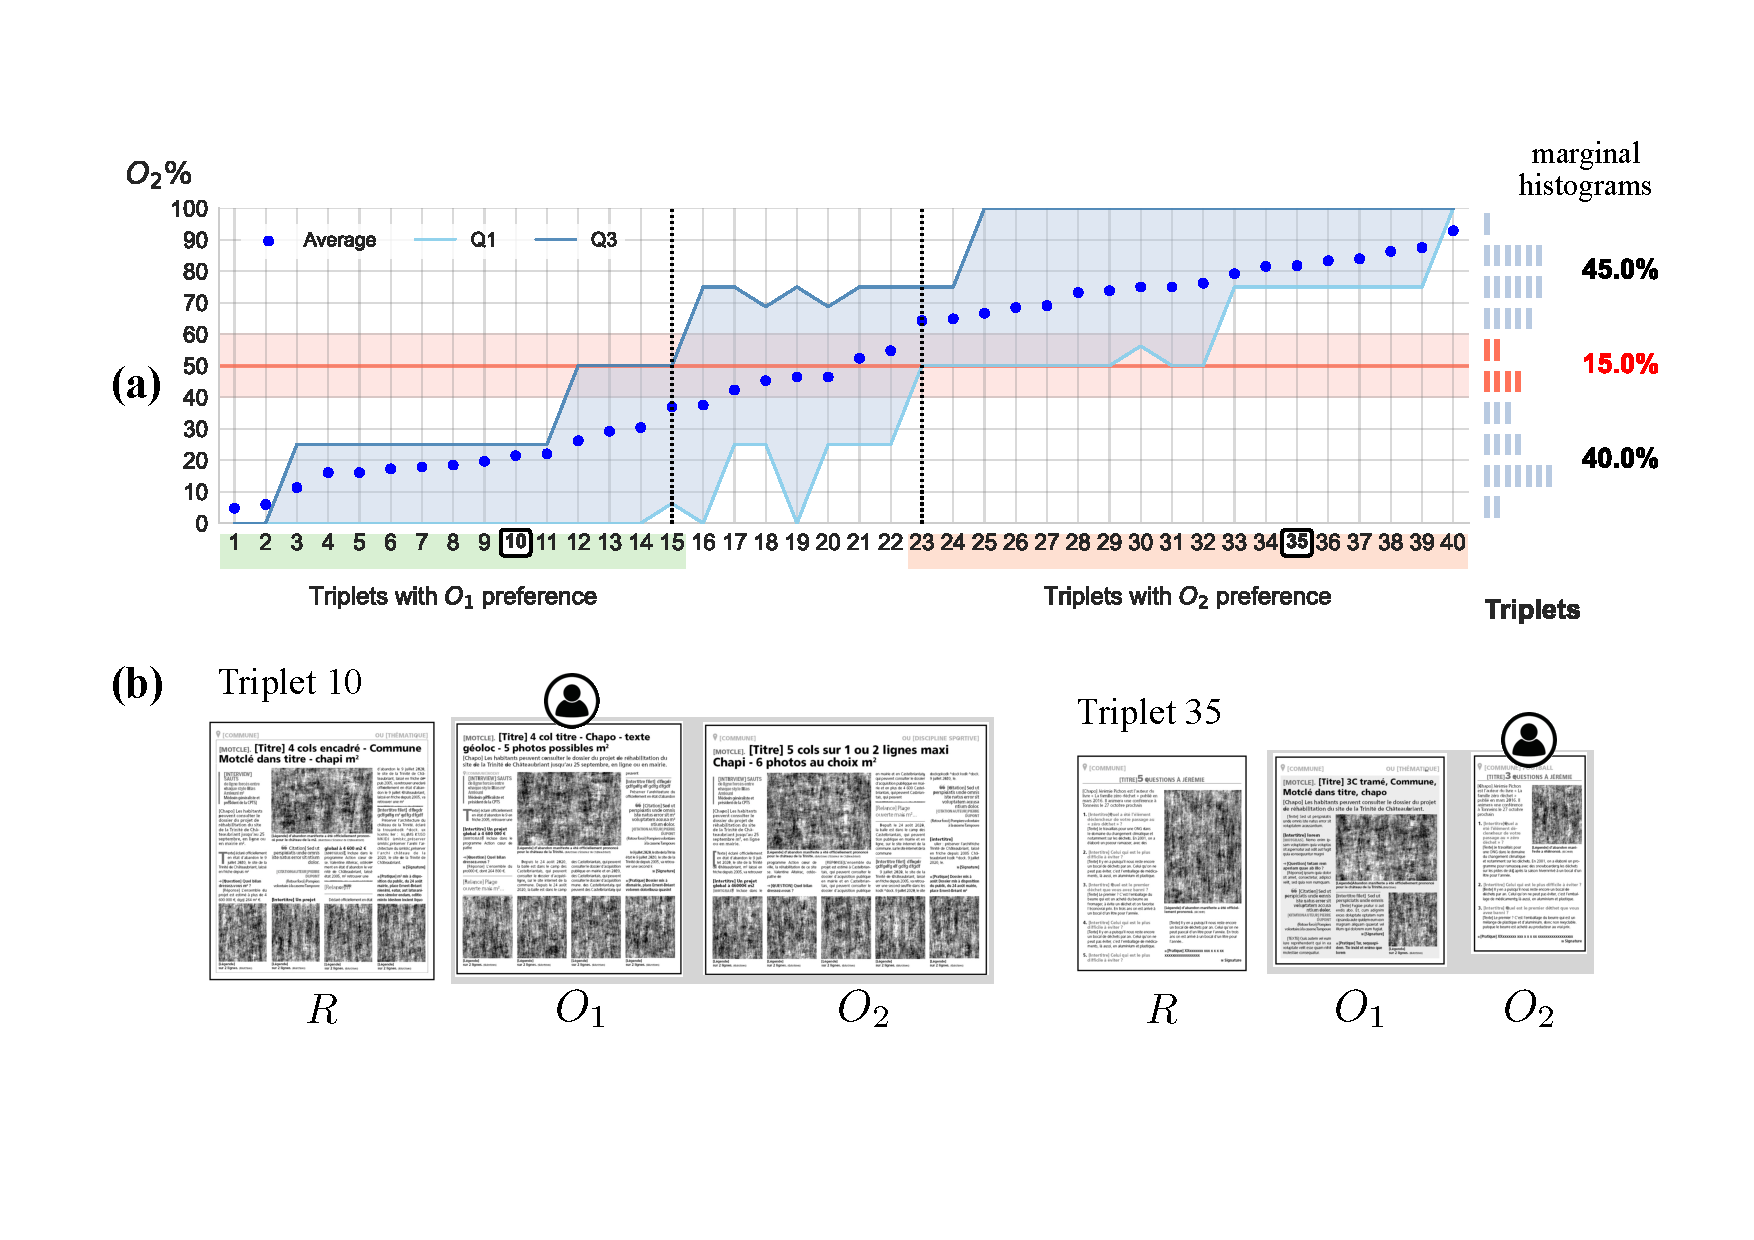
\includegraphics[width=\widthForOneImage]{img/online_experiment.pdf}
    \caption{\label{fig:online_experiment} 
Results of the online experiment.
(a) Percentage of $O_2$  selections for each of the 40 triplets. Each point represents the average percentage of $O_2$ selections, with the shaded area indicating the interquartile range ($Q1$–$Q3$). Two groups are highlighted: triplets \{1,\dots,15\} (green), where participants mainly selected $O_1$ ($\tdiou{\cdot}{\cdot}$), and triplets \{23,\dots,40\} (orange), where participants mainly selected $O_2$ ($\gmn{\cdot}{\cdot}$). A central band ($40\%$–$60\%$) where no clear preference was established. The marginal histogram (right) counts the frequency of triplets in $10\%$ intervals, where each block represents a single triplet. The bold percentage labels indicate the total proportion of the triplets falling into each of the three categories.
(b) Example triplets from each group. Individual participant choices are represented by a human-shaped icon.
    }
\end{figure}

\subsection{Qualitative comparison}
%todo complete this


This analysis lead to the selection of $\gmn{\cdot}{\cdot}$ as the main similarity measure to be used in this work.
%TODO maybe extend unless the previous section is conclusive enough

\section{Single-article template retrieval}
\label{section:template-retrieval-single-article}

\subsection{Problem formulation}
\label{sec:trs-problem-formulation}

Having established $\gmn{\cdot}{\cdot}$ as the primary metric for topological layout similarity in \secref{section:modelling-similarity}, this structural foundation can now be applied to solve automated template retrieval.

In the single article-per-article context, the template retrieval problem is defined as a top-$\topsize$ retrieval problem over a set of available templates $\templatecatalog$. Given a query content item and an extensive catalog of templates, the objective is to retrieve a small set of candidates that are both compatible with the content's technical constraints and structurally distinct from one another. A key requirement of this task is structural diversity: retrieved objects must vary significantly in their topological and spatial arrangements of internal components (e.g., text blocks, visual assets, titles) rather than representing minor geometric variations of the same underlying design template. A second critical requirement is novelty, or long-tail coverage~\cite{longtail}: traditional retrieval mechanisms in document repositories frequently rely on historical interaction statistics, favoring layouts that have been frequently selected in the past. While straightforward, this strategy introduces a severe popularity bias, creating a long-tail distribution where a small fraction of dominant designs are repeatedly retrieved, while a vast repository of potentially optimal and structurally unique alternatives remains underutilized. Together, these requirements echo strategies well documented in the Recommendation Systems (RS) literature~\cite{BOBADILLA2013109,vrijenhoek-diversity-2024}.


\begin{callout}
Despite this connection, the proposed setting is not a classical RS: traditional models are predominantly user-dependent, relying on collaborative filtering driven by historical interactions and individual user preferences, whereas the proposed definition of template retrieval is entirely user-agnostic and content-dependent, relying on objective structural characteristics. Likewise, the notion of diversity here applies directly to the topological layout structure rather than to historical consumption data. Consequently, in this section, classical recommendation concepts are adapted to a structurally grounded retrieval setting, where the goal is to optimize geometric coverage across the catalog.
\end{callout}

\subsection{Proposed approach}



% The framework operates in two complementary phases. In the offline phase, document layouts are modeled as graphs, and $\gmn{\cdot}{\cdot}$ is employed to organize the template catalog $\templatecatalog$ into clusters of structurally coherent designs. In the online query phase, the framework leverages these pre-computed clusters to perform diversity-aware retrieval for a given content item. Instead of treating retrieval as a flat ranking task, the mechanism samples candidate layouts across distinct structural clusters to compile the final results. This diversity-aware retrieval strategy is inspired by clustering-based diversification approaches in top-$\topsize$ recommendation~\cite{clusdiv}, adapted here to structured layout objects. In this architecture, $\gmn{\cdot}{\cdot}$ enables fine-grained structural comparisons, while diversity is explicitly enforced during the retrieval stage, ensuring that the returned top-$\topsize$ objects represent distinct architectural alternatives rather than minor variations of the same layout.

\subsubsection{Template Retrieval System (\trs) overview}
This framework is explicitly designed to promote structural diversity and novelty, enabling  broader range of distinct and potentially underused templates.

The proposed method takes as input the following elements:
\begin{itemize}
    \item A catalog of  templates $\templatecatalog$, where each template defines a layout composed of multiple content regions. Regions are represented as polygons (convex or concave, with or without holes) and are associated with semantic content types (e.g., text, image, title), as illustrated in \figref{fig:template}.
    
    \item A template usage log, recording how frequently each template has been used over a given time period. Templates that were not used during this period are assigned a usage value of zero, which in this context explicitly denotes absence of usage rather than missing or unknown feedback.
    
    \item Query content which define the subset of templates that are considered admissible (e.g., required number and types of content regions, size of text).
    
    \item The target number $\topsize$ of templates to obtain as output.
\end{itemize}

\trs is organized into two complementary components with distinct roles.
An offline component establishes a structural representation of the template catalog by learning similarities between templates and organizing them into clusters.
An online component constitutes the operational phase of the method: given a specific query content, it selects a small set of templates drawn from distinct clusters, ensuring both relevance and diversity in the proposed results. These two components are detailed in the following subsections.

\subsubsection{Offline component: catalog \templatecatalog\ clustering}

The objective of the offline component is to construct a structure-aware clustering over the template catalog, which serves as the foundation for diversity-aware selection at query time. This component operates entirely prior to any retrieval queries.

 Using the distance $d_{GMN}(\cdot,\cdot)$:
\begin{equation}
d_{GMN}(\templateobj{1},\templateobj{2}) = |\gmn{\templateobj{1}}{\templateobj{2}}|,
\label{eq:gmn-distance-definition}
\end{equation}
templates are organized via agglomerative clustering with a threshold $\clusterthreshold$, producing a set of clusters $\clusters$ (starting from singleton clusters, pairs of clusters are merged when their average inter-template distance is below $\clusterthreshold$).  Unlike methods such as ClusDiv~\cite{clusdiv}, the number of clusters is not tied to the target recommendation list size $\topsize$, but is determined solely by $\clusterthreshold$, which controls the tolerance for structural similarity of templates in the dataset. This clustering provides the foundation for the diversity-aware selection performed during the online retrieval phase.

\subsubsection{Online component: Template Retrieval Framework (\trf)}

In this phase, the set of  clusters $\clusters$ associated with the template catalog $\templatecatalog$ is already computed during the offline phase. The objective now is to generate, for a given query, a ranked list of $\topsize$ recommended templates that balances relevance, diversity, and novelty.
Each step of the method is presented incrementally, with reference to the pseudocode in Algorithm~\ref{alg:cw} and the illustration in \figref{fig:cw}. The process consists of three main stages: (1) Assign rating values, (2) Filter admissible templates, (3) Select templates for retrieval using cluster weights ($CW$) and diversity-aware mechanisms.
\begin{figure}[htbp]
    \centering
    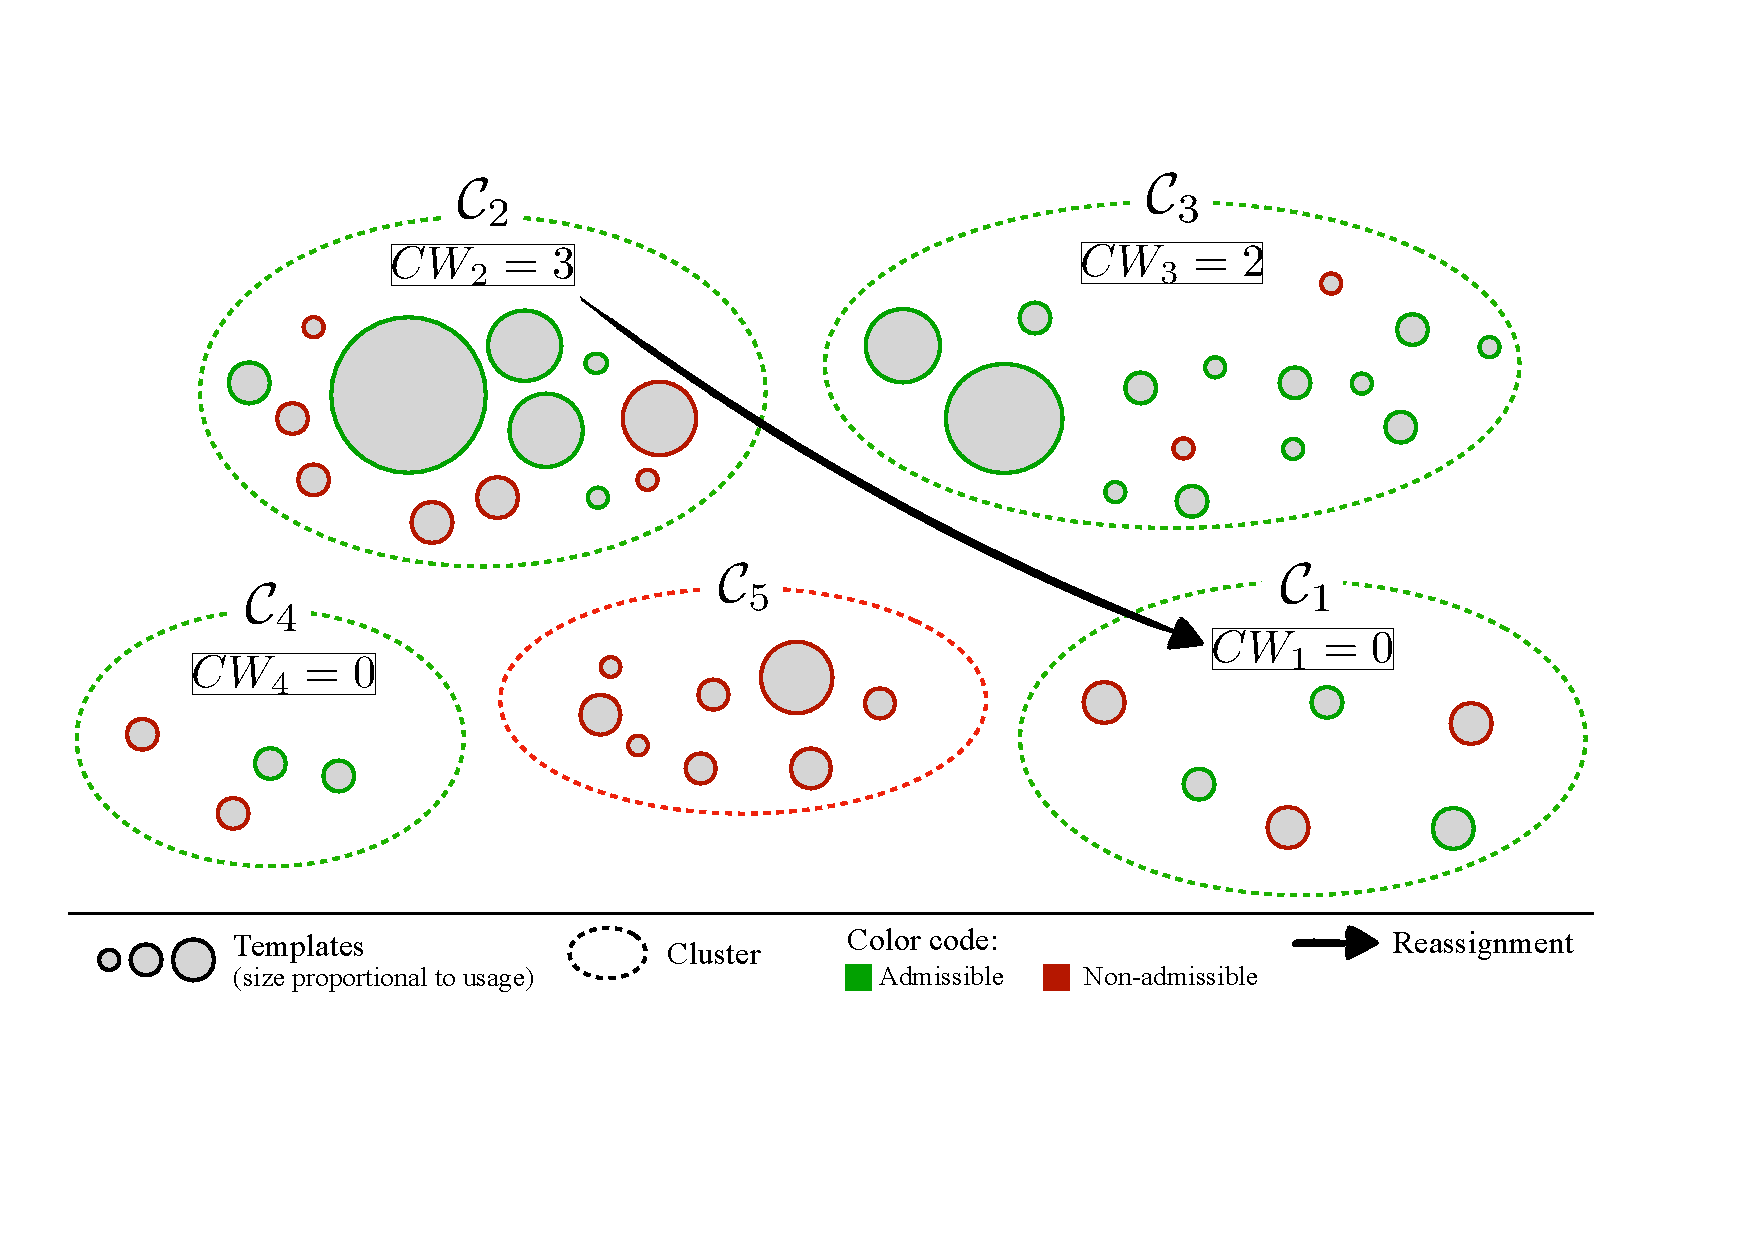
\includegraphics[width=\widthForOneImage]{img/our_trs_algorithm.pdf}
    \caption{\label{fig:cw} 
    Illustration of \trf under the assumption that $\cwthreshold < 3$. Each template is represented by a grey circle, with size proportional to its relative usage; templates are grouped into clusters outlined with dotted lines. Based on the input query, admissible templates are marked with green borders, while non-admissible templates have red borders. Cluster boundaries are also color-coded: clusters with at least one admissible template are marked in green, while those without (such as $\cluster{5}$) are marked in red. Using initial cluster weights, the reassignment algorithm first redirects weight values to $\cluster{2}$ until either $CW_2$ reaches the threshold $\cwthreshold$ or the maximum number of admissible templates in $\cluster{2}$ is reached. Subsequently, weights are also reassigned to $\cluster{1}$, given that it has the lowest $CW$ and the maximum distance from $\cluster{2}$. The final phase of the algorithm corresponds to the selection step, which recommends $CW_i$ templates per cluster $\cluster{i}$, prioritizing templates with the highest rating values (larger green circles) and applying a proximity penalty to reduce similarity among selected templates and further enhance diversity.
    }
\end{figure}

\begin{algorithm}
\caption{\label{alg:cw}Template Retrieval Framework (\trf) algorithm}
\begin{algorithmic}[1]
\REQUIRE \topsize: size of output list, $\cwthreshold$: diversity threshold, $\templatecatalog$: list of templates, $\{C_i\}$: list of clusters, usage of each template in $\templatecatalog$, input query.

\FOR{all templates $\templateincluster{i}{k}$ in each cluster $\cluster{i}$}
    \STATE assign rating value $r_{i,k}$ equal to usage of $\templateincluster{i}{k}$
\ENDFOR
\STATE $\admissibletemplates \leftarrow$ filtered $\templatecatalog$ based on requirements of the query (number of images, presence of title/subtitle, etc), sorted by $r_{i,k}$ in decreasing order.

\STATE Top-$\topsize$ $\leftarrow$ $\topsize$ templates in $\admissibletemplates$ with highest $r_{i,k}$.

\FOR{$n=1,...,N$ }
    \STATE $i \leftarrow $ cluster that contains template $n$ in the Top-$\topsize$ list. 
    \STATE $CW_i = CW_i + 1$ 
\ENDFOR

\FOR{\texttt{each source cluster }$\cluster{i}$ }
    \STATE $\admissibletemplatesincluster{i} \leftarrow$ set of admissible templates in cluster $i$
    \WHILE{$CW_i > \min \{|\admissibletemplatesincluster{i}|, \cwthreshold\}$} 
        \STATE $M = \{C_m\} \leftarrow$ set of clusters with $CW_m = \min_k CW_k$
        \STATE $C_j \leftarrow $ cluster with $\max_{C_m \in M} \min_{\templateincluster{i}{k} \in \admissibletemplatesincluster{i},\templateincluster{j}{l} \in \admissibletemplatesincluster{j}} \gmn{\templateincluster{i}{k}}{\templateincluster{j}{l}}$
        \STATE $CW_j = CW_j + 1$ 
        \STATE $CW_i = CW_i - 1$ 
    \ENDWHILE
\ENDFOR

\WHILE{$CW_i > 0$ for any $\cluster{i}$} 
    \STATE $\templateincluster{i}{k}$ $\leftarrow$ best template in $\admissibletemplates$ in terms of $r_{i,k}$
    \IF{$CW_i > 0$ }
        \STATE add $\templateincluster{i}{k}$ to output list
        \STATE $CW_i = CW_i - 1$
        \STATE Remove $\templateincluster{i}{k}$ from $\admissibletemplates$
        \FOR{all $\templateincluster{i}{l}$ where $GMN(\templateincluster{i}{k}, \templateincluster{i}{l}) < \gamma$}
            \STATE $r_{i,l} \leftarrow r_{i,l} / \kappa$ \COMMENT{$\kappa$ should be $\sim \infty$ }
        \ENDFOR
        \STATE Re-sort $\admissibletemplates$ in decreasing order of rating values $r_{i,l}$.
    \ELSE 
        \STATE Remove $\templateincluster{i}{k}$ from $\admissibletemplates$
    \ENDIF
\ENDWHILE

\STATE \textbf{Return:} output list.
\end{algorithmic}
\end{algorithm}


\paragraph{Stage 1: Assign rating values (Alg.~\ref{alg:cw}, lines 1--3)}
The first step in the online retrieval process is to assign a rating value to each template . Here, the rating corresponds directly to the usage history of the template. This provides a baseline measure of template popularity, which will guide the initial ranking.

This step ensures that frequently used templates are initially prioritized, while still leaving room for the algorithm to promote diversity and novelty in subsequent steps.

\paragraph{Stage 2: Filter admissible templates (Alg.~\ref{alg:cw}, line 4)}

The full template set $\templatecatalog$ was filtered according to the specified article requirements (e.g., presence of a title, number of images, or other structural constraints).

Formally, a template $\templateobj{j} \in \templatecatalog$ is classified as admissible, and thus included in the admissible subset $\admissibletemplates$, if and only if it simultaneously satisfies the following feasibility criteria:
\begin{itemize}
\item Image Allocation Integrity: The maximum image slot capacity of the template must accommodate the image count required by the article:
\begin{equation}
    \Nimg{i} \leq \Nimgmax{j}
\end{equation}

\item Title Consistency: The presence of a title element in the article must match the title block availability in the template:

\begin{equation}
\Tlart{i} = \Tltemp{j}
\end{equation}

\item Text Capacity Integrity: Assuming $\kactive{i} = \Nimg{i}$ active images are retained, the article's total character count $\Cart{i}$ must fall within the text capacity boundaries defined by the template's capacity matrix $\capacity{j}$, such that:  

\begin{equation}
    \capacity{j}[n_i, 0] \le c_i \le \capacity{j}[n_i, 1]
\end{equation}

\end{itemize}    


\paragraph{Stage 3: Cluster-weight–based template selection (Alg.~\ref{alg:cw}, lines 5--32)}

This stage determines how many templates should be selected from each cluster and then instantiates these selections while enforcing diversity constraints, using the similarity metric.

\paragraph{Initialize the $CW$ algorithm (Alg.~\ref{alg:cw}, lines 5--9)} 
The objective of this step is to initialize the number of templates to select from each cluster, and prepare the algorithm for the reassignment process. Following the notation of~\cite{clusdiv}, these quantities are denoted as cluster weights ($CW$), with one weight $CW_i$ associated to each cluster $\cluster{i}$.

Unlike the original ClusDiv formulation, the number of clusters is fixed and does not depend on the requested list size $\topsize$. However, the constraint $\sum_i CW_i = \topsize$ was enforced to guarantee that exactly $\topsize$ templates will be returned. We further assume that at least one admissible template exists; otherwise, the system trivially returns an empty set.

The initialization proceeds as follows. Given the admissible template set $\admissibletemplates$, first it extracts the top-$\topsize$ templates ranked by their rating values. Then, all cluster weights are initialized to zero and then increments $CW_i$ for each occurrence of a template belonging to cluster $\cluster{i}$ in this top-$\topsize$ list.

This initialization reflects the natural distribution induced by the highest-rated admissible templates, providing a starting allocation that is consistent with usage-driven preferences while remaining agnostic to diversity considerations, which are addressed in the subsequent reassignment stage.

\paragraph{Reassign cluster weights for diversity (Alg.~\ref{alg:cw}, lines 10--18)}
The purpose of this step is to redistribute cluster weights in order to increase diversity across the retrieval list.
Starting from the initial $CW_i$ values obtained from the Top-$\topsize$ templates, the algorithm iteratively reassign weights from over-represented clusters to under-represented ones.

To achieve this, the original $CW$ algorithm defined in~\cite{clusdiv} was adapted to consider only admissible templates. A key assumption in Algorithm~\ref{alg:cw} is that parameter $\topsize$ is smaller than $\admissibletemplates$. If not, the algorithm simply outputs all admissible templates. 

A critical feature of this algorithm is the selection process for increasing  $CW_j$ in cluster $j$ from a source cluster $i$. Here the clusters with the highest priority are the ones with the smallest $CW_j$ that contain admissible templates, breaking ties by selecting the farthest cluster $j$ based on the distance function $d_{tGMN}(.)$. This is illustrated in \figref{fig:cw}

This distance is determined by calculating the maximum distance between all admissible templates in the source cluster $i$ and those in target cluster $j$. This procedure ensures increased diversity in the retrievals by considering the greatest distance between clusters.

\paragraph{Template Selection (Alg.~\ref{alg:cw}, lines 19--31)}
In the final section of the algorithm, templates are selected from the admissible set according to the cluster weights $\{CW_i\}$ computed in the previous step. The goal is to construct a retrieval list of size $\topsize$ that respects both relevance, driven by usage, and structural diversity across clusters.

At each iteration, the algorithm considers the admissible template with the highest rating value.
If this template belongs to a cluster $\cluster{i}$ with $CW_i > 0$, it is added to the output list and the corresponding cluster weight is decreased by one. Otherwise, the template is skipped. This process is repeated until all cluster weights are exhausted.

To further promote local diversity,  a local suppression mechanism was introduced, inspired by diversification strategies in recommendation systems.
After selecting the $k$-th template $\templateincluster{i}{k}$ in cluster $\cluster{i}$, the rating values of all remaining templates $\templateincluster{i}{l}$ in the same cluster that are structurally too similar are penalized.
More precisely, and given two templates $\templateincluster{i}{k}$ and $\templateincluster{i}{l}$ from the same cluster $i$; if $d_{tGMN}(t_{i,k}, t_{i,l}) < \gamma$, the rating value $r_{i,l}$ is divided by a factor $\kappa$. Both parameters were set through empirical pilot studies, with $\kappa$ chosen sufficiently large to strongly inhibit near-duplicate layouts.
This suppression prevents the immediate selection of highly similar templates while keeping them available for later iterations if needed.

At the end of this process, the proposed method returns a ranked list
\[
\recolist{N} = [\templateincluster{k_1}{i_1}, \templateincluster{k_2}{i_2}, \dots, \templateincluster{k_N}{i_N}],
\]
that balances usage-driven relevance with structural diversity and novelty.


\subsection{Experimental evaluation}
\label{section:trs-eval}
%%%%%%%%%%%%%%%%%%%%%%%%%%%%%%%%%%%%%%%%%%%%%%%%%%%%%%%%%%%%%%%%%%%%%%%%
\subsubsection{Template Catalog Dataset}
%%%%%%%%%%%%%%%%%%%%%%%%%%%%%%%%%%%%%%%%%%%%%%%%%%%%%%%%%%%%%%%%%%%%%%%%
The template repository $\templatecatalog$ utilized in this evaluation is derived from the \publihebdos template archive (\secref{sec:publihebdos}).

%\footnotetext{With the permission of PubliHebdos, the templates were cleaned and anonymized before being released as a research dataset. The repository, together with template usage metadata, is publicly available at: \url{https://anonymous.4open.science/r/Newspaper-Template-Dataset-EFEF/}}.

%%The repository was curated to ensure consistency, completeness, and shareability.

%Each template is represented by (1) a JSON description encoding the layout structure, as formalized in Chapter~\ref{chapter:definitions}, and (2) a visual preview generated with synthetic text and randomized image placeholders (see examples in \figref{fig:template-example}). 

%Table~\ref{tab:dataset-info} summarizes the main characteristics of the repository, while \figref{fig:dataset-info-graphs} reports distributions over key layout properties, including the number of columns, number of images, and aspect ratios. Together, these statistics illustrate the structural diversity of the template repository.

%In addition, the usage statistics associated with each template reveal a highly imbalanced distribution.  
%A small subset of templates accounts for the majority of historical usage, while approximately $17\%$ of templates have never been used. More than $90\%$ of templates have fewer than $1{,}600$ recorded uses, indicating a pronounced long-tail distribution. The observed properties transcend this specific repository, appearing consistently across multiple catalogs within the same CMS. 

%Such imbalance increases the risk of catalog stagnation and motivates the need for diversity- and novelty-aware selection mechanisms.

%\begin{table}[htbp]
 %   \centering
 %   \begin{tabular}{lc}
   %    \hline
  %  Description & Value\\
   % \specialrule{.2em}{.1em}{.1em}
    %    Number of templates & 452 \\
    %    Average width (mm) & 137.1  \\
   %      Average height (mm) & 132.9  \\
   %     Average number of images & 1.48\\
  %      Average number of different classes & 3.29\\
  %      Average number of columns & 3.19\\
  %  Template ID with max usage & 3142 \\
 %   Max usage & 38005\\
  %  Number of Zero-usage templates & 79 \\
  %  Average usage & 781.8\\
  %  Usage deviation & 3433.4\\
  %   \% templates with usage $<1600$ & 92\% \\
   %  \% templates with usage $<8000$ & 96\% \\
   %  \hline
  %  \end{tabular}
   % \caption{Table with general information about the dataset.}
   %% \label{tab:dataset-info}
%\end{table}

 %\begin{figure}[htpb]
  %   \centering
  %   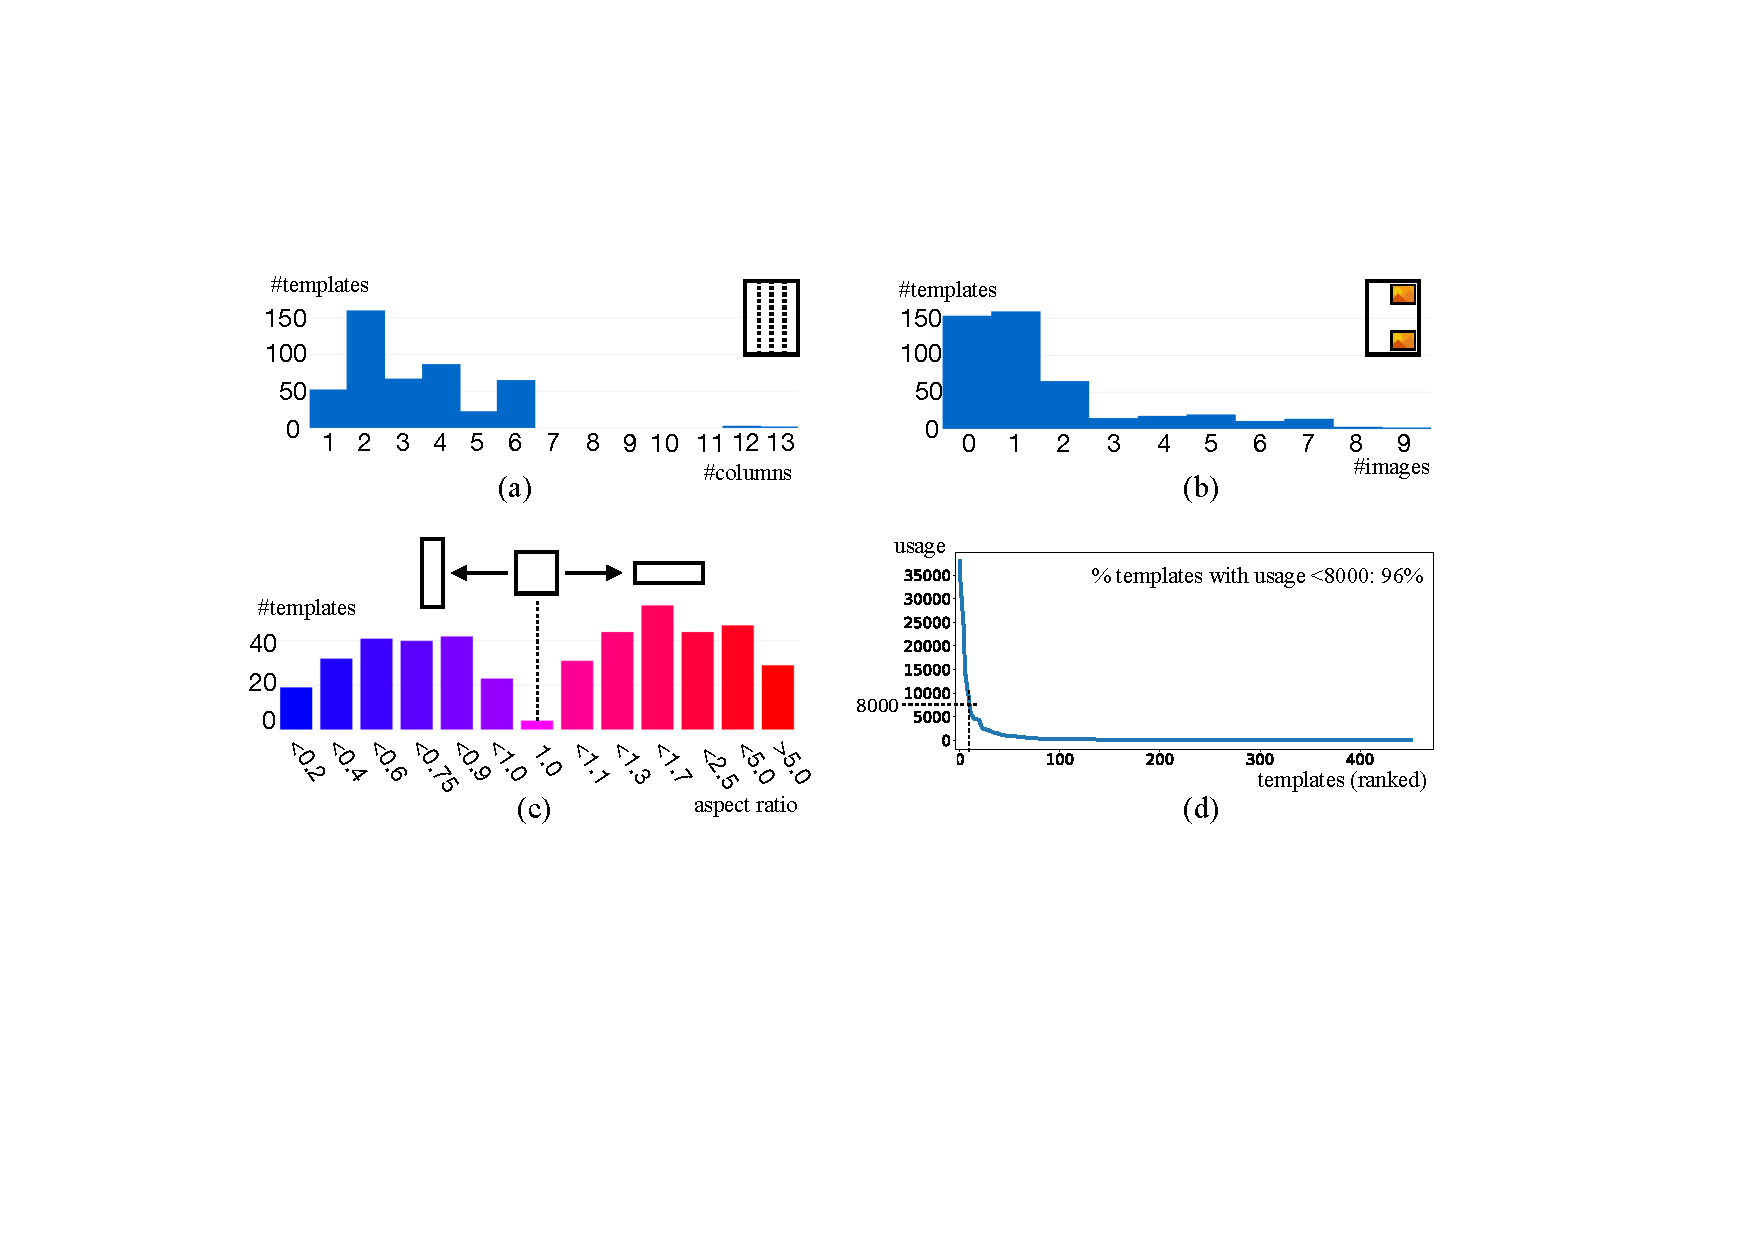
\includegraphics[width=\widthForOneImage]{img/dataset_info_general.pdf}
   %  \caption{
   %  Overview of template dataset characteristics: 
   %  (a) distribution of column counts per template, 
   %  (b) distribution of image counts within templates,  
   %  (c) distribution of template aspect ratios, and 
    % (d) usage distribution of templates, reordered by decreasing usage, during a 7-month period. These plots provide a general overview of the structural and usage diversity in the repository. 
   % }
    % \label{fig:dataset-info-graphs} 
 %\end{figure}

 \subsubsection{\gmnNetwork training and clustering results}
 \label{sec:gmn-training}
 \paragraph{\gmnNetwork training.}
The first task is to train the LayoutGMN network used to measure structural similarity between templates.
To generate the training data,  an augmented version of the template repository $\templatecatalog$ was generated, denoted $\extendedtemplates$. For each template containing images,  all possible variants obtained by removing $i = 0,1,\ldots,n$ images were generated, thereby creating additional space for body text. This augmentation strategy preserves the overall layout structure while introducing controlled geometric variability.
As a result, the augmented dataset $\extendedtemplates$ contains 5,341 templates.

\gmnNetwork is trained on $\extendedtemplates$ using the triplet-based framework described in~\cite{patil_layoutgmn_2021}. During training, care is taken to ensure that no template appears simultaneously in the training and test sets within any triplet. The main training parameters, set through empirical pilot studies, are reported in Table~\ref{tab:params}. With this configuration, the network achieves 98\% accuracy on the test set. This performance is comparable to that reported in~\cite{patil_layoutgmn_2021}, confirming the ability of the model to capture structural isomorphism between layouts. These results validate the use of the learned embedding distance as a reliable similarity measure for the subsequent clustering stage.
\begin{table}[htbp]
    \centering
    \begin{tabularx}{\textwidth}{@{}l l X l@{}}
    \toprule
    Category & Symbol & Parameter Description & Value \\
    \midrule
    \multirow{5}{*}{\gmnNetwork training}
               & --- & Batch size & 20 \\
               & --- & Epochs & 500 \\
               & --- & Dataset size & 5341 \\
               & --- & Training set size & 80\% \\
               & --- & Validation set size & 20\% \\
    \midrule
    Clustering & $\clusterthreshold$ & Distance threshold for agglomerative clustering & $2.8$ \\
    \midrule
    \multirow{2}{*}{Online selection}
               & $\gamma$ & Structural similarity threshold for local suppression & $0.5$ \\
               & $\kappa$ & Rating penalization factor for near-duplicate templates & $10^7$ \\
    \bottomrule
    \end{tabularx}
    \caption{Main parameters used across similarity learning, clustering, and online selection.}
    \label{tab:params} 
\end{table}

\paragraph{Template clustering.}
The structural similarity function learned by LayoutGMN is then used as a distance metric to perform agglomerative clustering over the original template repository. Using the clustering threshold set through preliminary pilot studies and reported in Table~\ref{tab:params}, a total of 81 clusters was obtained.

\figref{fig:cluster-graphs} presents an analysis of the resulting clusters in terms of both size (number of templates per cluster) and cumulative usage. This reveals that the majority of isolated clusters are concentrated near the origin, representing singletons—clusters containing a single template—with minimal cumulative usage. These points correspond to highly specialized layouts with distinctive geometries that are rarely reused in practice. Conversely, the progression toward the upper-right quadrant identifies a smaller subset of clusters that dominate usage statistics. A deeper analysis revealed that these high-usage clusters, including the highlighted outlier, effectively group generic templates, such as text-only layouts, single-image templates, or standard image-with-caption configurations of varying sizes. 

This clustering structure makes explicit the distinction between generic layouts and rare, specialized ones. This organization is essential for diversity-aware contexts, as it enables the system to compare and select templates within and across structurally coherent groups, instead of relying on usage statistics alone.


\begin{figure}[htbp]
    \centering
    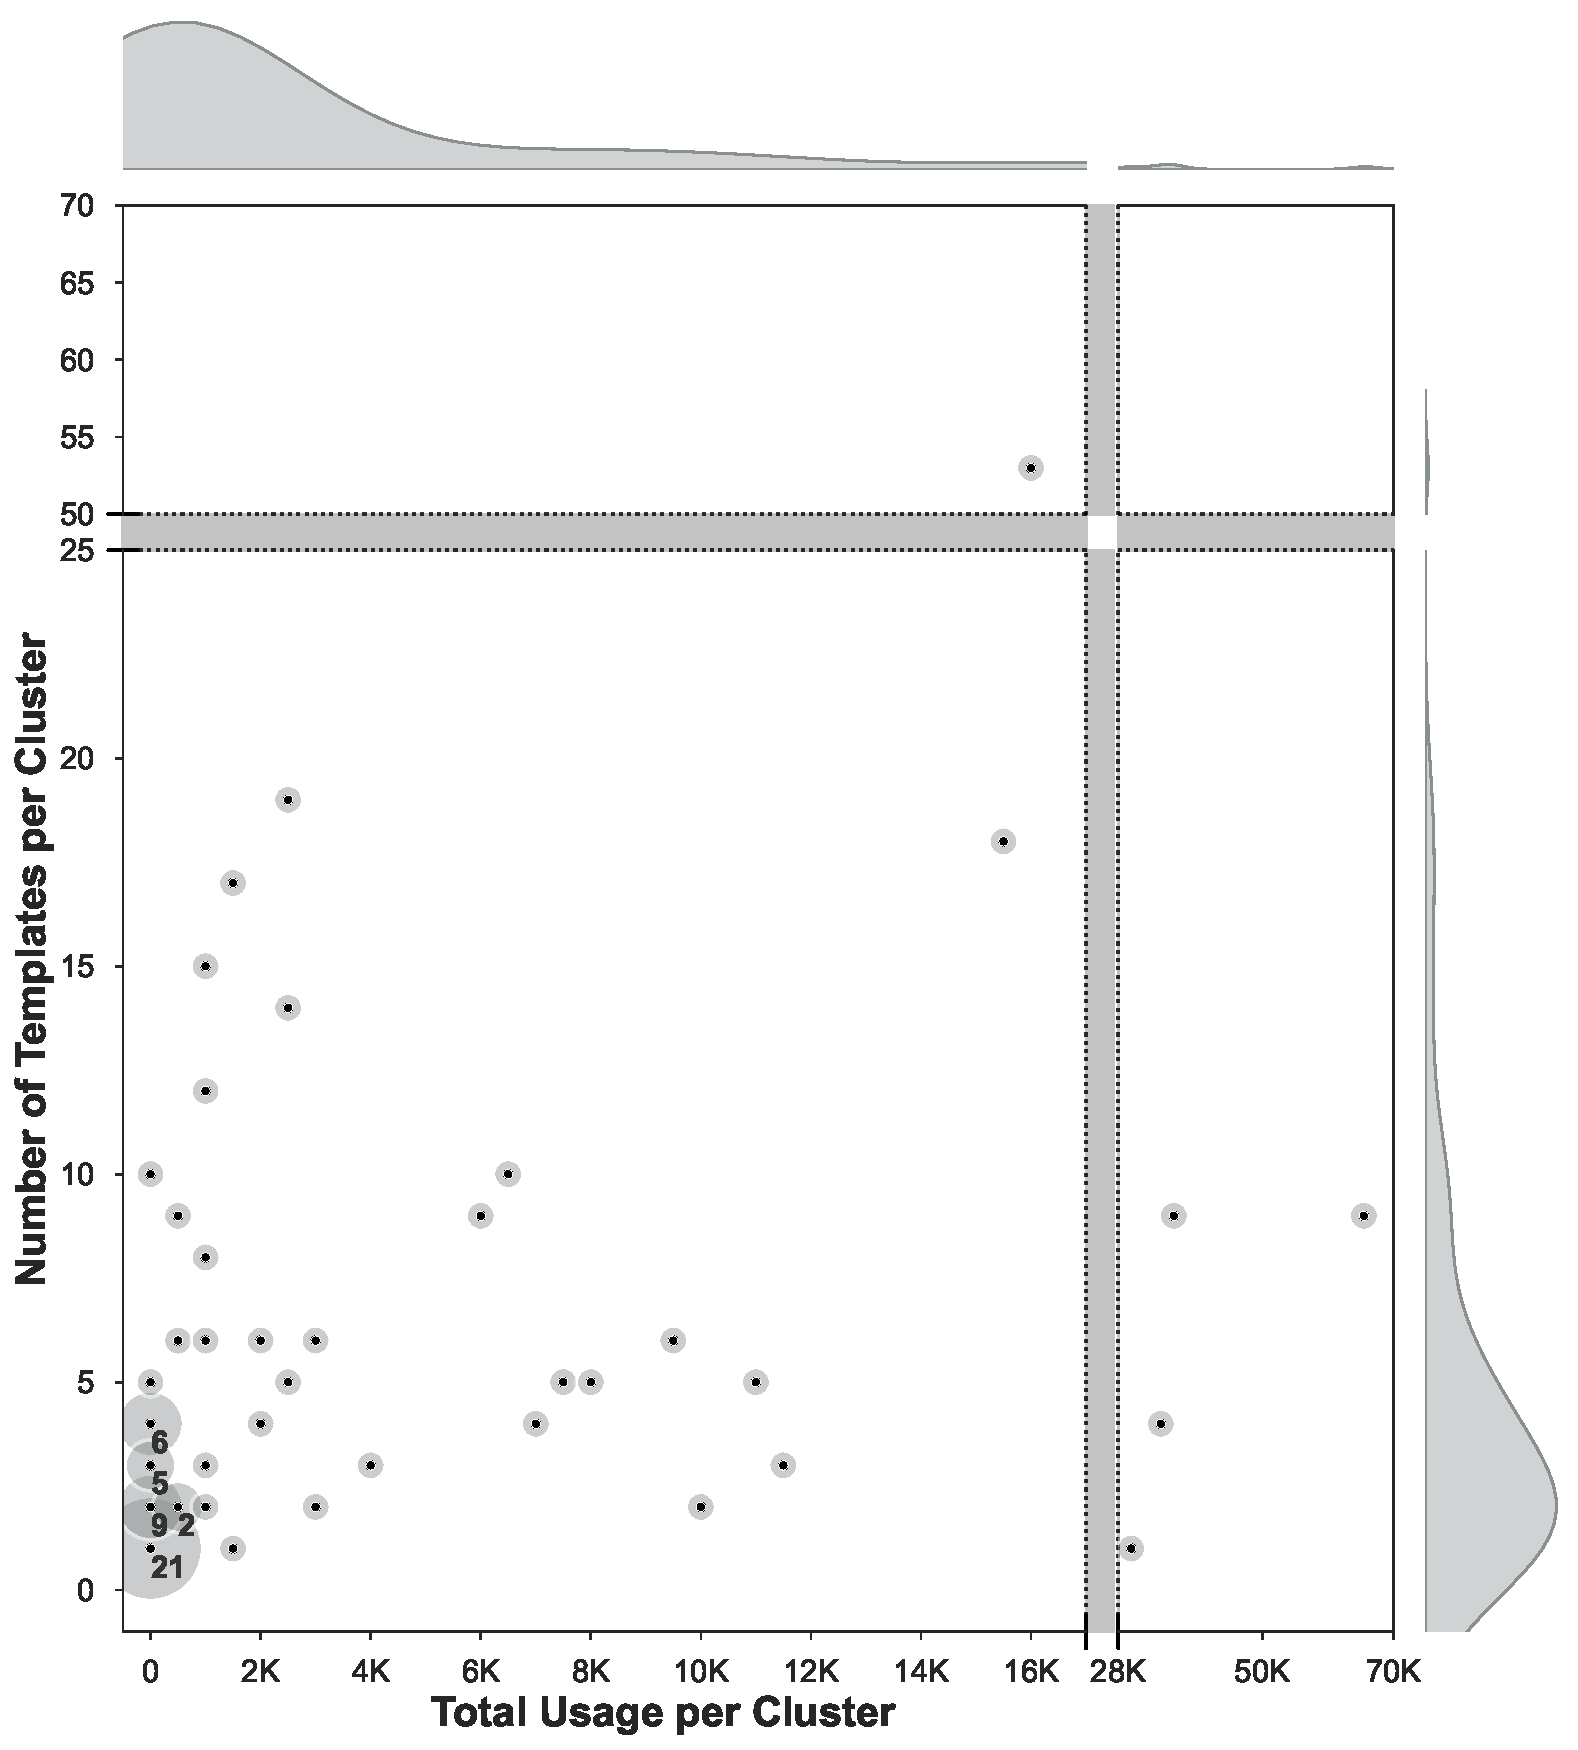
\includegraphics[width=\widthForOneImage]{img/templates_x_usage_x_histograms.pdf}
    \caption{
    Cluster distribution analytics by total usage and template count.
    Each black point indicates the presence of at least one cluster sharing those specific characteristics. To visualize cluster density, data is grouped into  bins of 500 units of total usage, represented by overlaid bubbles. The size of these bubbles denote the number of clusters in each case. Numerical labels provide the exact cluster count for each bubble (if absent, corresponds to a single cluster). To maintain visual clarity of the graph, the visualization employs a dual broken-axis scale (indicated by shaded zones and guide lines). Additionally, marginal distribution plots (KDE) on the top and right axes highlight frequency peaks, visually confirming that the vast majority of clusters are concentrated in the lower-left quadrant.
    }
    \label{fig:cluster-graphs}
\end{figure}

%%%%%%%%%%%%%%%%%%%%%%%%%%%%%%%%%%%%%%%%%%%%%%%%%%%%%%%%%%%%%%%%%%%%%%%%
\subsubsection{Evaluation of the Online Template Selection}
%%%%%%%%%%%%%%%%%%%%%%%%%%%%%%%%%%%%%%%%%%%%%%%%%%%%%%%%%%%%%%%%%%%%%%%%

In this section, the performance of \trs during the online phase is evaluated. 
The main goal is to generate candidate template lists that primarily respect historical editorial usage while also promoting structural diversity and enabling exploration of less frequently used templates. 

Accordingly, the evaluation was led along three central dimensions: 
(1) \emph{conformity to historical usage}, capturing how well the selected templates align with past editorial behavior; 
(2) \emph{structural diversity}, measuring the variety of layouts in the selection; and 
(3) \emph{long-tail exposure}, also known as novelty, reflecting the ability to surface underutilized templates. 
Additionally, the computational efficiency was reported as a secondary measure of practical relevance.


\paragraph{Observed and Synthetic Template Usage Distributions for Evaluation}
%%%%%%%%%%%%%%%%%%%%%%%%%%%%%%%%%%%%%%%%%%%%%%%%%%%%%%%%%%%%%%%%%%%%%%%%

First, it is necessary to examine how template usage is distributed across structural clusters in $\templatecatalog$. In addition to the nominal observed distribution, a controlled synthetic distribution was  designed to evaluate the robustness of diversification mechanisms under unfavorable popularity–structure correlations.
These two distributions are illustrated in \figref{fig:cluster-usage}.
\begin{figure}[htbp]
    \centering
    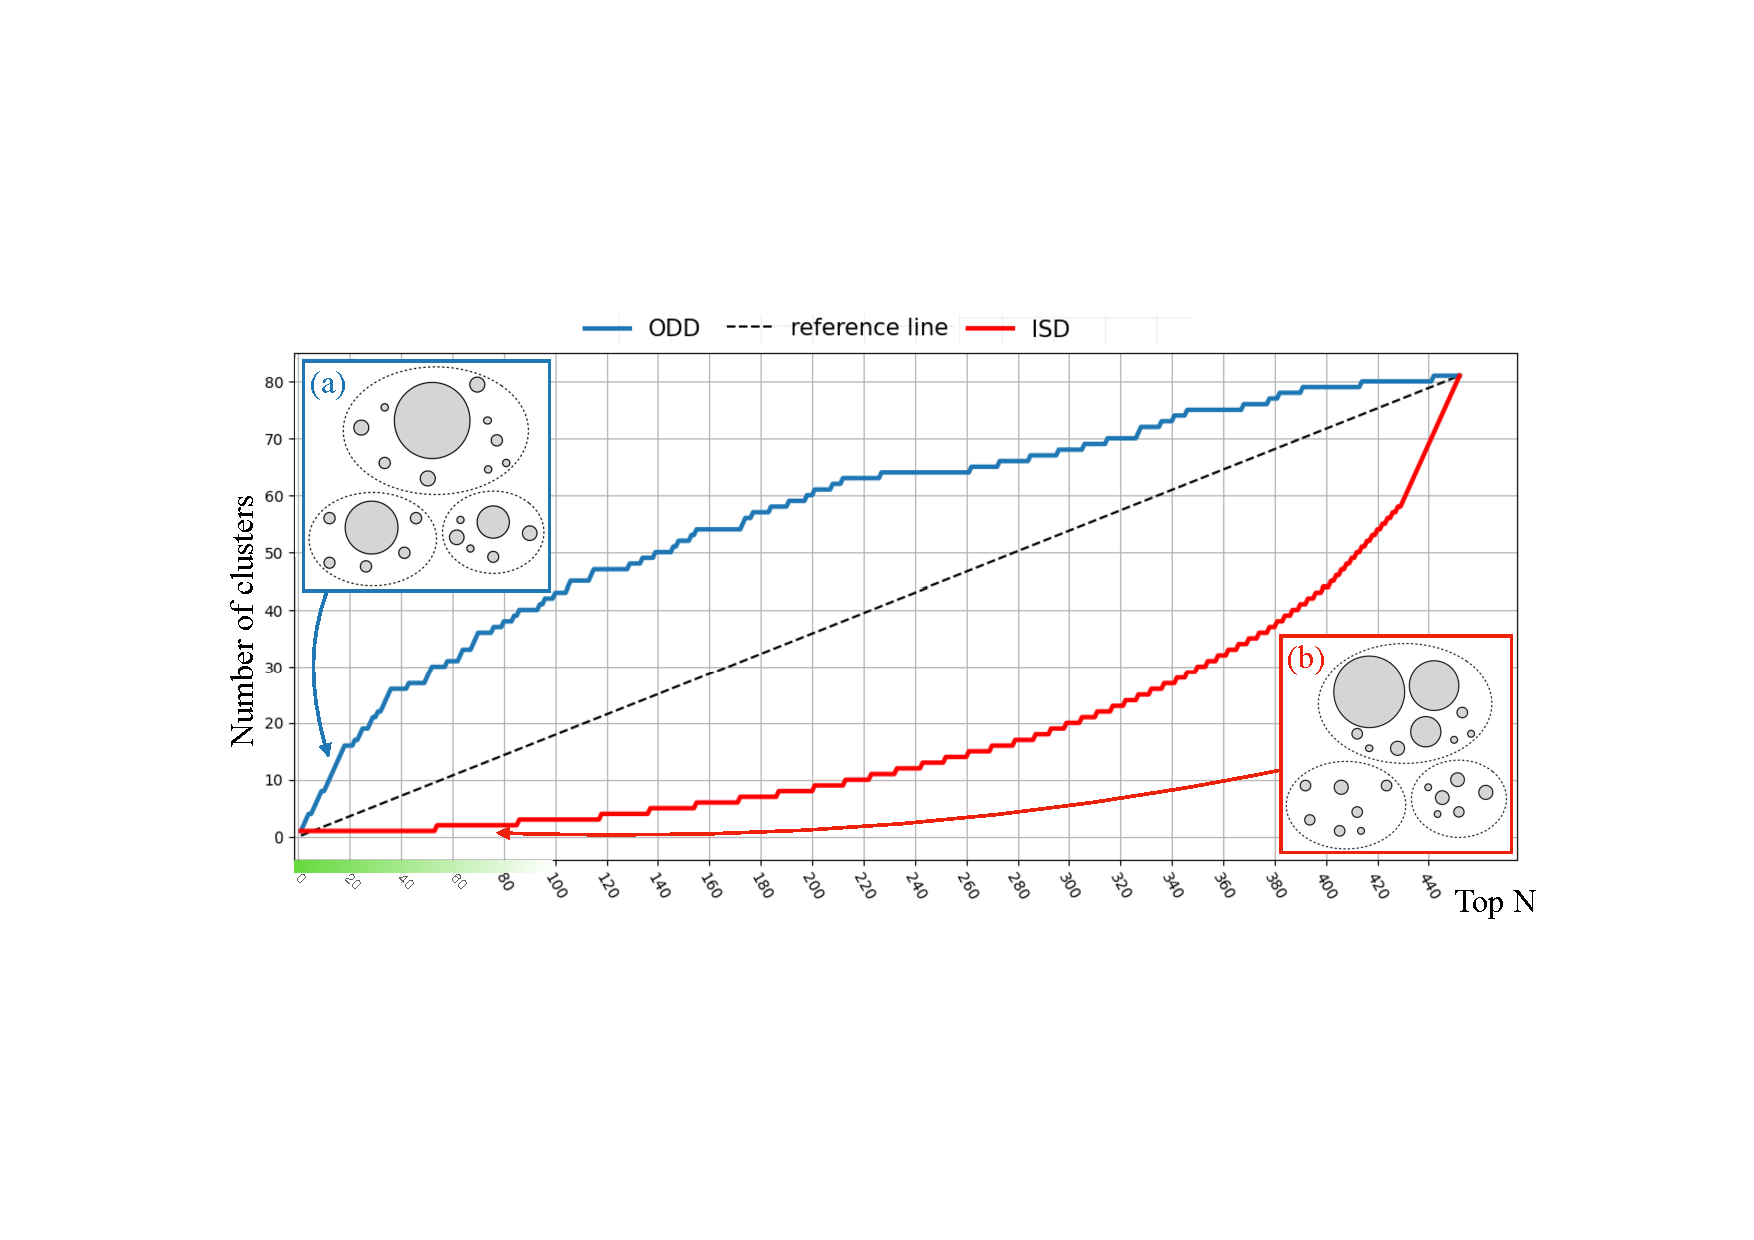
\includegraphics[width=\widthForOneImage]{img/cluster_usage.pdf}
    \caption{
   Observed and Synthetic Template Usage Distributions. This figure shows the number of clusters used to group the top-$\topsize$ templates (ranked by usage) for two distinct distribution scenarios. The first scenario, represented by the blue curve, corresponds to the \emph{Original Dataset Distribution} (\ODD), where top-$\topsize$ templates are more evenly distributed across clusters, particularly for low $\topsize$-values (green region). This spread suggests that selecting templates based on usage alone should yield satisfactory diversity. The second scenario, shown by the red curve, simulates a situation where high-usage templates are more frequently concentrated within the same clusters and is termed the \emph{Increasing Slope Distribution} (\ISD). This arrangement is intentionally designed to be nearly symmetric relative to the dotted reference line, creating a more challenging scenario, as selecting templates based solely on usage would likely lead to lower diversity in the output.}
   \label{fig:cluster-usage}
\end{figure}

\begin{itemize}
    \item[\textbf{Original Dataset Distribution (\ODD)}] This distribution corresponds to the cumulative number of clusters used to group the top-$\topsize$ templates according to their original usage values. The short head of the distribution (e.g., the top-20 most-used templates) is relatively dispersed across distinct clusters.
This property is favorable for popularity-driven selection strategies, as selecting high-frequency templates may already yield a non-trivial level of structural diversity.

\item[\textbf{Increasing Slope Distribution (\ISD)}] To evaluate diversity performance under less favorable conditions,  a synthetic distribution was constructed, in which highly used templates are deliberately concentrated within the same structural clusters. Specifically, clusters are first sorted in decreasing order of size. Usage values are then reordered independently in decreasing order and reassigned to templates within these clusters, ensuring that the most frequently used templates are grouped together. This synthetic setting is coined as \emph{Increasing Slope Distribution} (\ISD), reflecting its characteristic shape in \figref{fig:cluster-usage}. This distribution simulates a clustered popularity effect, where structural similarity and high usage are strongly correlated, thereby creating a challenging evaluation context for diversity-aware selection mechanisms.

In the remainder of this section,  all methods were evaluated on the same template repository $\templatecatalog$, using the original usage values under \ODD and the reassigned usage values under \ISD.
\end{itemize}



%%%%%%%%%%%%%%%%%%%%%%%%%%%%%%%%%%%%%%%%%%%%%%%%%%%%%%%%%%%%%%%%%%%%%%%%
\paragraph{Baseline Methods}
%%%%%%%%%%%%%%%%%%%%%%%%%%%%%%%%%%%%%%%%%%%%%%%%%%%%%%%%%%%%%%%%%%%%%%%%

To evaluate the effectiveness of \trs, three baseline strategies were proposed for a performance comparison. Table~\ref{tab:baselines_summary} summarizes the key differences between features of the baselines in comparison to the proposed framework.
\begin{itemize}
    \item[\textbf{Most Popular (\mostpopular)}] This simple baseline outputs the \topsize most frequently used templates in the admissible set. It serves as a reference for conformity to historical usage and reflects current and common industrial practice.
    \item[\textbf{Classic ClusDiv (\classicclusdiv)}] A state-of-the-art clustering-based method. Templates are clustered according to historical usage, using the number of clusters equal to the top-\topsize list. 
Unlike our approach, this method does not have a specific heuristic for choosing which cluster with the minimum $CW_i$ (cluster weight) will increase during each iteration. To account for this, we run the algorithm with five different random seeds to select the cluster with minimum $CW_i$, producing five distinct versions of the same algorithm for comparison.

\item[\textbf{Adapted ClusDiv (\adaptedclusdiv)}] To bridge the gap between \classicclusdiv and \trs, \adaptedclusdiv is introduced as an ablation baseline. While \classicclusdiv fixes the number of clusters to \topsize and ignores structural similarity, this adaptation incorporates $\gmn{\cdot}{\cdot}$ structural distance for clustering and allows for a flexible number of clusters. However, it retains all other properties of \classicclusdiv: (1) it lacks a heuristic for selecting among clusters with identical minimum $CW_i$ during iterations, and (2) it does not include an intra-cluster suppression mechanism. Consequently, \adaptedclusdiv serves to isolate and evaluate the specific impact of the retrieval logic. 
Following the protocol of \classicclusdiv, the same five random seeds weer used to resolve ties when selecting clusters with the minimum $CW_i$.
\end{itemize}



\begin{table}[htbp]
    \centering
    \begin{tabular}{lcccc}
        \toprule
        \textbf{Method} & \textbf{CB}  & \textbf{SM}  & \textbf{NI}  & \textbf{SL} \\
        \midrule
        \mostpopular    & $\times$     & $\times$     & --           & $\times$    \\
        \classicclusdiv & $\checkmark$ & $\times$     & $\times$     & $\times$    \\
        \adaptedclusdiv & $\checkmark$ & $\checkmark$ & $\checkmark$ & $\times$    \\
        DSTS            & $\checkmark$ & $\checkmark$ & $\checkmark$ & $\checkmark$ \\
        \bottomrule
        %\multicolumn{5}{l}{\footnotesize $^*$Selection heuristic between clusters with minimum $CW_i$ and intra-cluster suppression.}
    \end{tabular}
\caption{
Comparison of features across baseline methods and \trs.
Abbreviations: CB = clustering-based; SM = uses a similarity measure for clustering; NI = number of clusters independent of \topsize; SL = selection logic, corresponds to the selection heuristic between clusters with minimum $CW_i$ and intra-cluster suppression. }
\label{tab:baselines_summary}
\end{table}

%%%%%%%%%%%%%%%%%%%%%%%%%%%%%%%%%%%%%%%%%%%%%%%%%%%%%%%%%%%%%%%%%%%%%%%%
\paragraph{Evaluation Metrics}
%%%%%%%%%%%%%%%%%%%%%%%%%%%%%%%%%%%%%%%%%%%%%%%%%%%%%%%%%%%%%%%%%%%%%%%%


Performance is evaluated along the three core dimensions identified previously: conformity to historical usage, structural diversity and long-tail coverage. 
To simplify notations, and since the cluster index is no longer important in the final candidate template list,  the retrieved list is denoted as $\recolist{N} = [\templateobj{i_1}, \templateobj{i_2},..., \templateobj{i_N}]$. 

\begin{itemize}
    \item[\textbf{Conformity to Historical Usage}] \emph{Normalized Discounted Cumulative Gain} ($nDCG$) was used to measure alignment with historical usage. Relevance is defined by each template’s usage. $nDCG$ compares the ordering of the candidate template list to the ideal ordering (MostPopular list), yielding a score in $[0,1]$, where 1 indicates perfect conformity.

More precisely, the normalized Discounted Cumulative Gain ($nDCG$) evaluates how well the ordering of templates in the candidate list aligns with an ideal ranking based on historical usage. In this context, the relevance of a template $\templateobj{i}$ is given by its historical usage $\templateutilization{i}$, and the candidate list of selected templates is denoted by $\recolist{N}$.
First, it is necessary to define the Discounted Cumulative Gain ($DCG$) of the list $\recolist{N}$ as:
\[
    DCG@N(L) = \sum^{N}_k \templateutilization{k} / \log_2(k+1).
    %\label{eq:dcg}   % not used
\]
where $\templateutilization{k}$ is the usage of the template at position $k$ in $\recolist{N}$. The logarithmic denominator penalizes templates with high usage that appear lower in the list, reflecting the importance of ranking more frequently used templates toward the top.

The normalized DCG is then computed as:
\[
    nDCG@N = \frac{DCG@N (\recolist{N})}{DCG@N (L'(N))},
    %\label{eq:ndcg}   % not used
\]
where $L'$ corresponds to the ranking given by the \mostpopular algorithm, which orders templates in decreasing order of historical usage. By construction, $nDCG$ ranges from $0$ to $1$, with $1$ indicating perfect conformity to historical usage. This formulation allowS to quantify, in a normalized manner, how well the candidate list respects past preferences.


\item[\textbf{Structural Diversity}] To measure structural diversity related to the topological differences between the elements in $\recolist{N}$, \emph{absolute diversity} metric~\cite{clusdiv} was used, computed as the average pairwise $\gmn{\cdot}{\cdot}$ distance ($d_{tGMN}$) between templates in the list:
\[
D(L) = \frac{1}{N(N-1)} \sum_{\templateobj{i} \in \recolist{N}} \sum_{\templateobj{j} \in \recolist{N}, i \neq j} d_{tGMN}(\templateobj{i},\templateobj{j}),
\]
Higher values indicate more diverse layouts. This metric focuses on absolute structural variation without reference to the dataset distribution.

\item[\textbf{Long-Tail Coverage}] Analyzing the usage distribution of templates, reordered by decreasing usage (see \figref{fig:dataset-info-graphs}(d)), an usage $\templateutilization{k}$ threshold of $8000$ is defined to distinguish between the short head and the long tail. To assess a method's ability to retrieve templates beyond the top 4\% of the most frequently used ones, the \emph{long-tail percentage} (\LTP) for a retrieval list $\recolist{N}$ can be calculated as the proportion of templates in $\recolist{N}$ with usage $\templateutilization{k}$ below $8000$.
\end{itemize}




%%%%%%%%%%%%%%%%%%%%%%%%%%%%%%%%%%%%%%%%%%%%%%%%%%%%%%%%%%%%%%%%%%%%%%%%
\paragraph{Performance Analysis} 
%%%%%%%%%%%%%%%%%%%%%%%%%%%%%%%%%%%%%%%%%%%%%%%%%%%%%%%%%%%%%%%%%%%%%%%%

This section evaluates the online template retrieval framework (\trf) of \trs under different operating conditions. The objective is not only to quantify algorithmic performance, but also to assess how \trf behaves in realistic scenarios, where the number of proposed templates and the level of enforced diversity may vary.

Two parameters govern the behavior of the selection process:  
(i) the list size $\topsize$, which corresponds to the number of candidate templates to retrieve and is therefore application-driven; and  
(ii) the cluster weight threshold $\cwthreshold$, which controls the maximum number of templates selected per cluster and acts as an internal diversification constraint.

 Each parameter was varyed in turn, while fixing the other to a representative value. This allows to (i) characterize the trade-offs induced by diversity mechanisms and (ii) verify the robustness of the proposed approach across different usage regimes. This evaluation also considers both observed and synthetic template usage distributions, namely \ODD and \ISD distributions. 
 
 To rigorously benchmark the retrieval framework under maximum search space complexity and prevent trivial candidate pruning, all experimental evaluations were conducted without applying specific admissibility constraints. Consequently, the full template catalog was treated as completely admissible ($\admissibletemplates = \templatecatalog$)

 Results are shown in \figref{fig:performance-analysis-three-criteria} and commented below.

\begin{figure}[htbp]
    \centering
    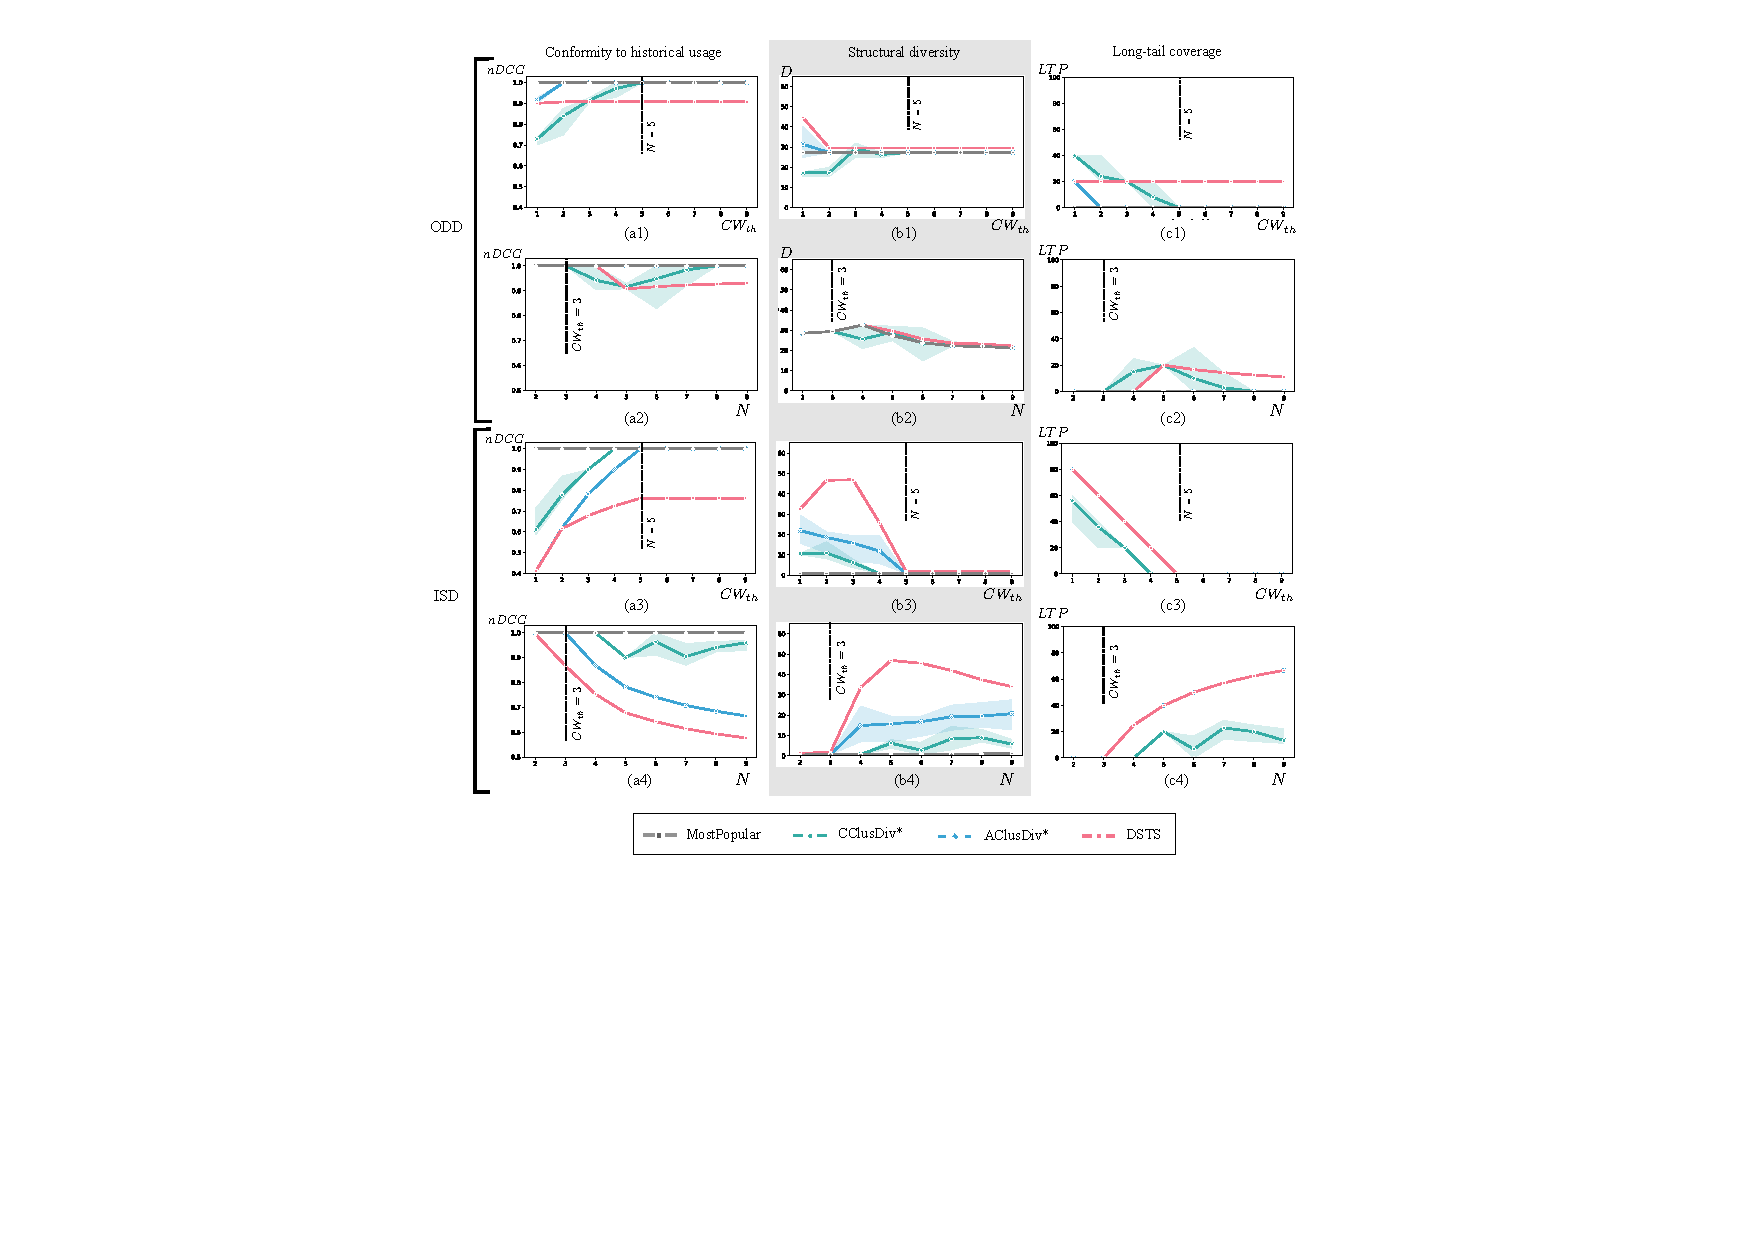
\includegraphics[width=\widthForOneImage]{img/performance-analysis-three-criteria.pdf}
    \caption{
    Performance evaluation across three criteria.
Columns correspond to evaluation metrics:
(a) Conformity to historical usage,
(b) Structural diversity,
(c) Long-tail coverage.
Rows correspond to distribution scenarios and parameter settings:
rows 1–2: ODD, rows 3–4: ISD;
odd rows: fixed $\topsize$, varying $\cwthreshold$;
even rows: fixed $\cwthreshold$, varying $\topsize$.
    Methods with multiple variants (\classicclusdiv and \adaptedclusdiv) are represented by their average values (colored dots) and a shaded region indicating the range. These methods are marked with a star (*) in the legend. The black dashed lines indicate the boundary where $\cwthreshold = \topsize$. Beyond this point ($\cwthreshold \geq \topsize$), the metrics for all algorithms stabilize as no further $\cwthreshold$ reassignments occur. Instances where a curve is not apparent implies that the corresponding data is flat and coincident with the horizontal axis ($y=0$). }

    \label{fig:performance-analysis-three-criteria}
\end{figure}

First, it is necessary to analyze conformity to historical usage, measured using $nDCG$, because before promoting diversity or novelty, it is essential to verify that the proposed method does not excessively deviate from the historical conformity.

\figref{fig:performance-analysis-three-criteria}(a1) and (a3) report $nDCG$ values as a function of $\cwthreshold$ for a fixed list size $\topsize=5$. As expected, increasing diversification constraints leads to a gradual decrease in conformity for all diversity-aware methods. This effect is more pronounced for our approach due to the local suppression mechanism, which deliberately penalizes templates that are structurally too similar to previously selected ones.

Importantly, this decrease remains controlled across both the Original Dataset Distribution (\ODD) and the more challenging Increasing Slope Distribution (\ISD). While \mostpopular trivially achieves the maximum $nDCG$, it does so at the expense of diversity, as commented in the next section. In contrast, \trs  maintains acceptable conformity levels while enabling substantially richer template sets. This behavior reflects the intended compromise: historical usage is respected as a baseline, but not enforced as the sole decision criterion.

Similar trends are observed when varying \topsize with fixed $\cwthreshold=3$ (\figref{fig:performance-analysis-three-criteria}(a2) and (a4)). Notably, \classicclusdiv exhibits a sharper degradation in $nDCG$ when $\cwthreshold < \topsize$, as clustering by usage forces the selection of very low-frequency templates during reassignment. \trs avoids this abrupt drop by decoupling structural similarity from usage during clustering.


Now it is turn to measure structural diversity, which constitutes the primary objective of \trs.
For fixed $\topsize=5$, \figref{fig:performance-analysis-three-criteria}(b1) and (b3) show that under the \ODD case, \trs achieves slightly higher diversity than baseline approaches. This gain is mainly attributable to the local suppression mechanism, which prevents the selection of near-duplicate layouts within the same cluster.

Under the \ISD case, the advantage becomes substantial. Here, the cluster weight reassignment strategy plays a critical role: by reallocating selection capacity toward structurally distant clusters, the method significantly increases diversity compared to all baselines. As shown in \figref{fig:performance-analysis-three-criteria}(b3) and (b4), \trs reaches a structural diversity score near $40$, whereas baseline methods peak at around $20$ for the same parameters, effectively doubling ($2x$) the diversity.

An interesting behavior emerges as $\cwthreshold$ varies. For small values, repeated reassignment steps progressively increase local diversity by encouraging exploration across distant clusters. Beyond a certain point, however, excessive relaxation of the constraint leads to a convergence toward more similar templates, causing diversity to plateau or decrease. This effect highlights the existence of an operational regime where diversity gains are maximized without over-fragmenting the selection.

When varying \topsize with fixed $\cwthreshold=3$ (\figref{fig:performance-analysis-three-criteria}(b2) and (b4)), the same trends persist. Diversity typically peaks when $N \approx 2\cwthreshold$, confirming that \trs scales coherently with the size of the output list.


Finally, and beyond structural diversity,  \trs ability to promote underutilized templates is analyzed, measured using \LTP (\figref{fig:performance-analysis-three-criteria}(c1--c4)).

The \mostpopular baseline systematically selects templates from the short head of the distribution, resulting in zero long-tail coverage. \classicclusdiv exhibits high long-tail usage for small $\cwthreshold$, but this effect rapidly diminishes as the constraint relaxes. \adaptedclusdiv, which does not cluster by usage, shows limited ability to surface rare templates.

In contrast, \trs consistently retrieves at least one low-usage template under the \ODD scenario (\figref{fig:performance-analysis-three-criteria}(c1) and (c3)), regardless of $\cwthreshold$, due to the combined effect of cluster-level diversification and local suppression . Under \ISD (\figref{fig:performance-analysis-three-criteria}(c2) and (c4)), long-tail coverage remains higher than for all baselines across the full range of parameters. Furthermore, the results in \figref{fig:performance-analysis-three-criteria}(c3) and (c4) indicate a improvement of approximately $1.5x$ over the baselines. This advantage tends to diminish for large $\cwthreshold$, as fewer constraints are available to force the exploration of low-usage regions.

These results confirm that the proposed selection mechanism does not merely redistribute diversity among frequent templates, but actively contributes to catalog exploration.

\paragraph{Execution Time}
Additionally, the execution time is measured to assess whether \trs meets the latency requirements of editorial workflows.
Execution time is measured as a function of \topsize for fixed $\cwthreshold=3$ (\figref{fig:time_cw3}). For clarity, only this configuration was reported, as varying $\cwthreshold$ yields similar trends.
\trs incurs additional computational cost compared to \adaptedclusdiv due to inter-cluster distance evaluations during reassignment. However, both methods remain significantly faster than \classicclusdiv, which performs clustering at runtime. Although execution time increases for \ISD when $\topsize > \cwthreshold$, it remains in the millisecond range, making it suitable for deployed systems that implements \trs.

\begin{figure}[htbp]
    \centering
    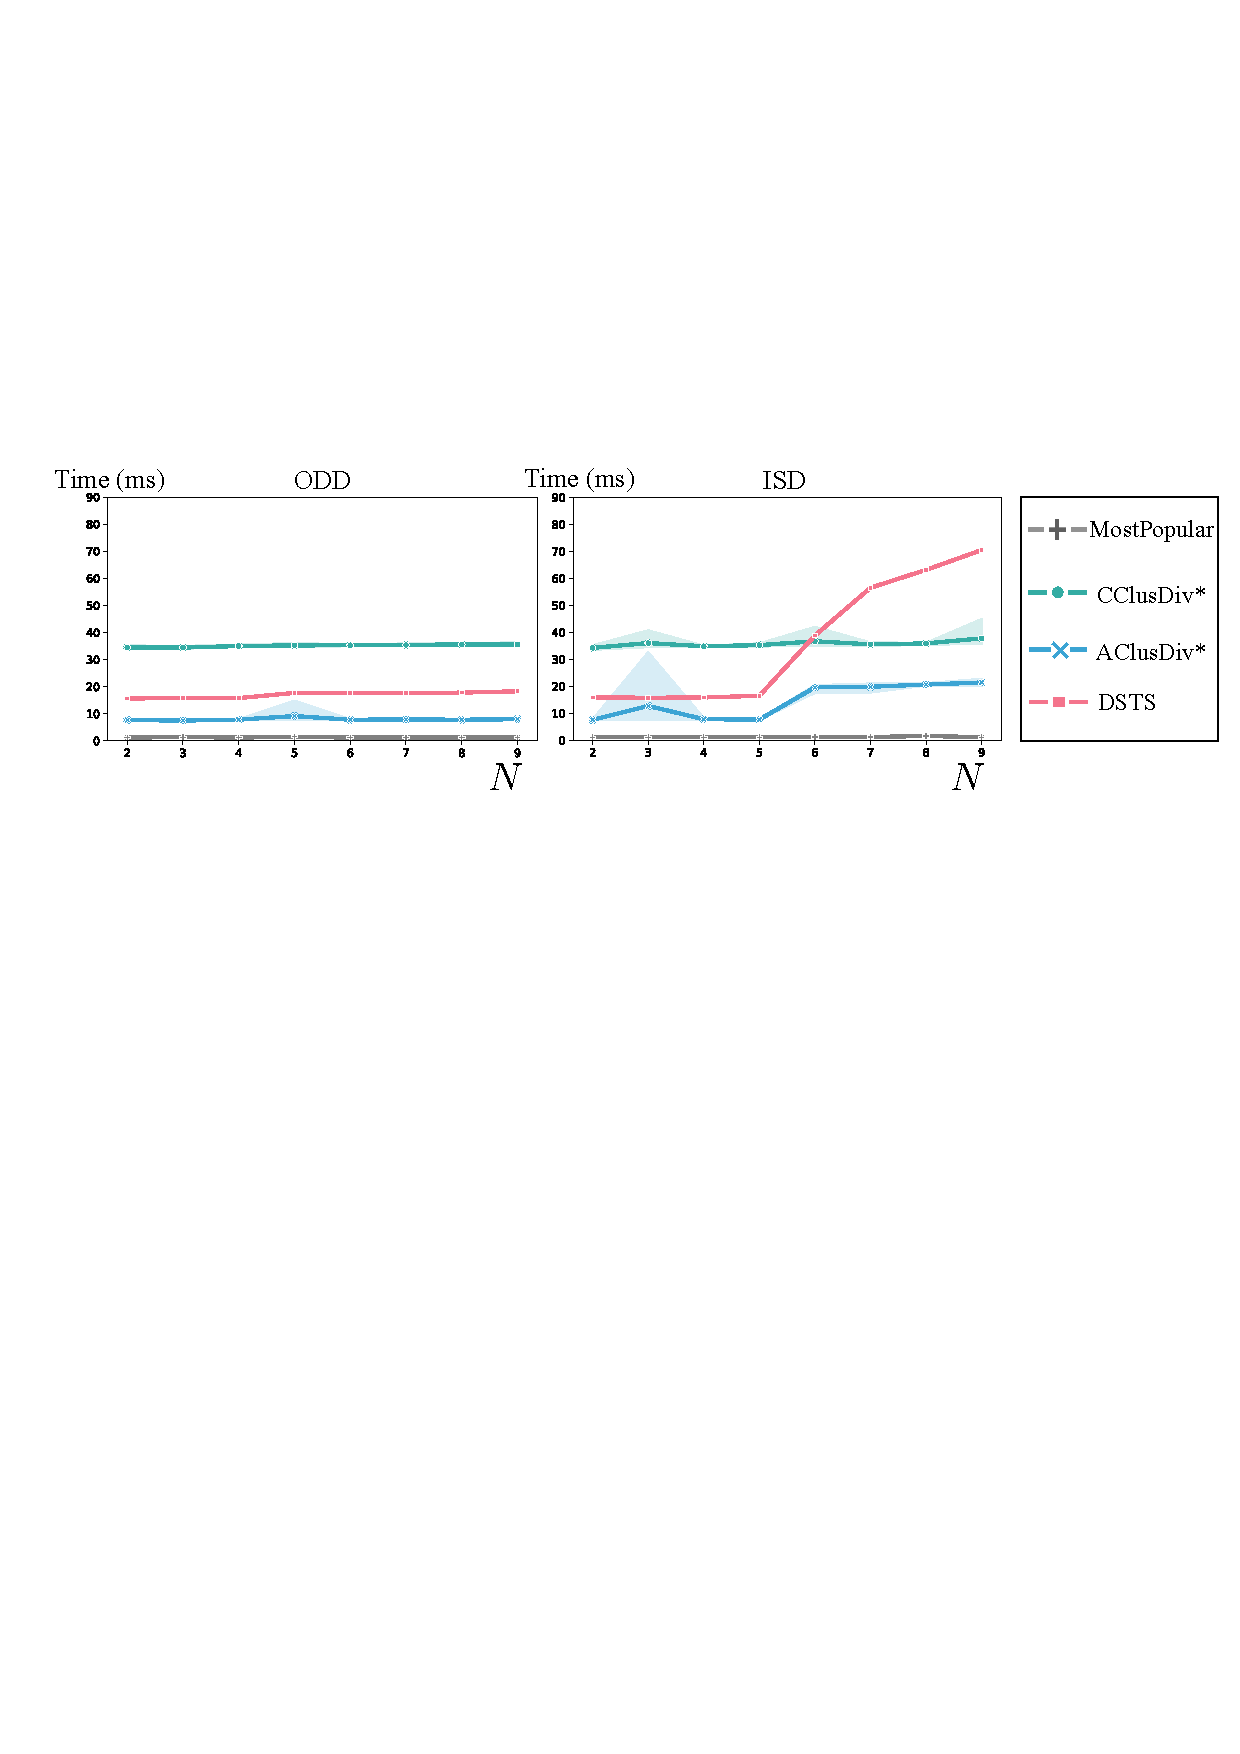
\includegraphics[width=0.9\widthForOneImage]{img/time.pdf}
    \caption{
    Execution Time: Time vs \topsize for fixed $\cwthreshold=3$ for both observed and synthetic template usage distributions.
    }
    \label{fig:time_cw3}
\end{figure}

%%%%%%%%%%%%%%%%%%%%%%%%%%%%%%%%%%%%%%%%%%%%%%%%%%%%%%%%%%%%%%%%%%%%%%%%
\subsubsection{Example Outputs}
%%%%%%%%%%%%%%%%%%%%%%%%%%%%%%%%%%%%%%%%%%%%%%%%%%%%%%%%%%%%%%%%%%%%%%%%
\figref{fig:example-1} and \figref{fig:example-2} present the top-$5$ retrieved templates from two different query examples, illustrating the performance of \trs compared to baseline methods. Note that templates are arranged in a specific order to facilitate comparison across methods, rather than their actual ranking (which follows a decreasing order of usage). All examples were generated using $\cwthreshold = 2$. Additionally, a frame around each template is included to assist in size comparison.
\begin{figure}[htbp]
    \centering
     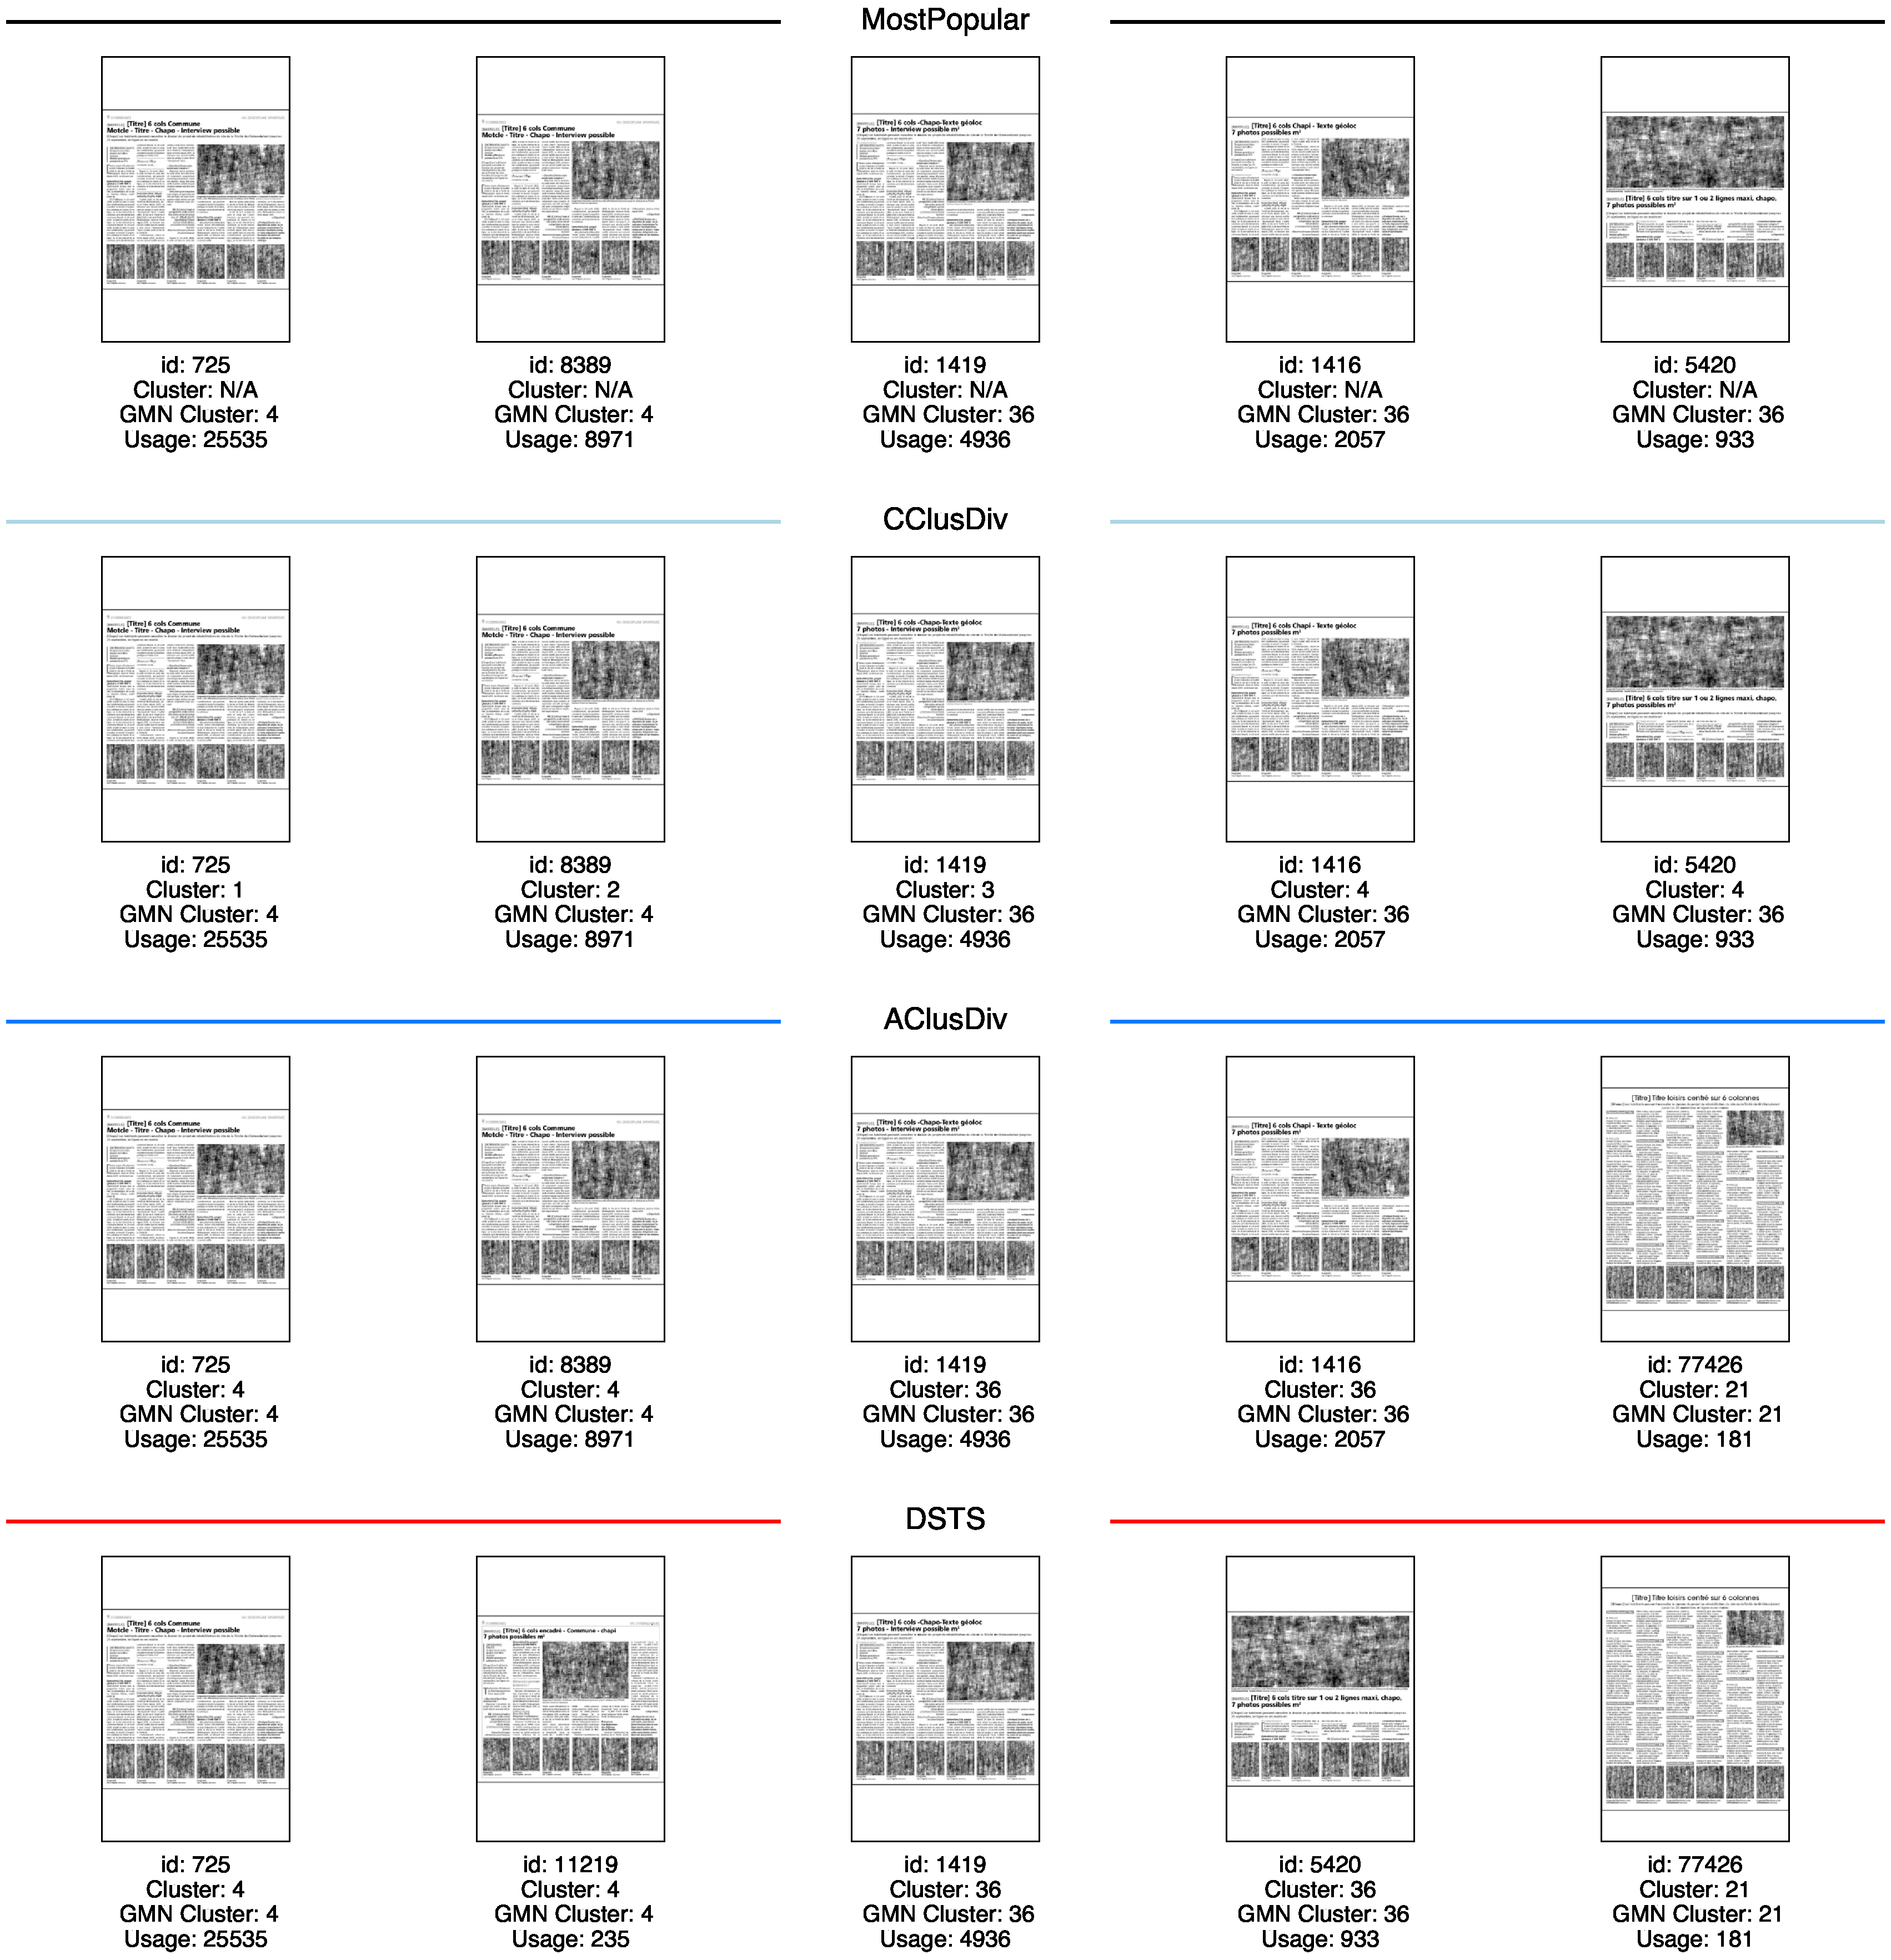
\includegraphics[width=\widthForOneImage]{img/example_prompt_ex_1.pdf}
    \caption{
    Comparison of the top 5 recommended templates with one title and seven images, given by baseline methods and \trs. IDs, corresponding clusters (if applicable), and usage are reported. Additionally, the GMN-based cluster is indicated for comparison.
    The figure highlights how our method improves diversity not only through similarity-based clustering (as in \adaptedclusdiv) but also by promoting intra-cluster diversity (e.g., IDs 11219 and 5420) via the suppression mechanism. Usage values further demonstrate that our method enhances novelty (\LTP) compared to baseline methods.
    }
    \label{fig:example-1} 
\end{figure}
\begin{figure}[htbp]
    \centering
     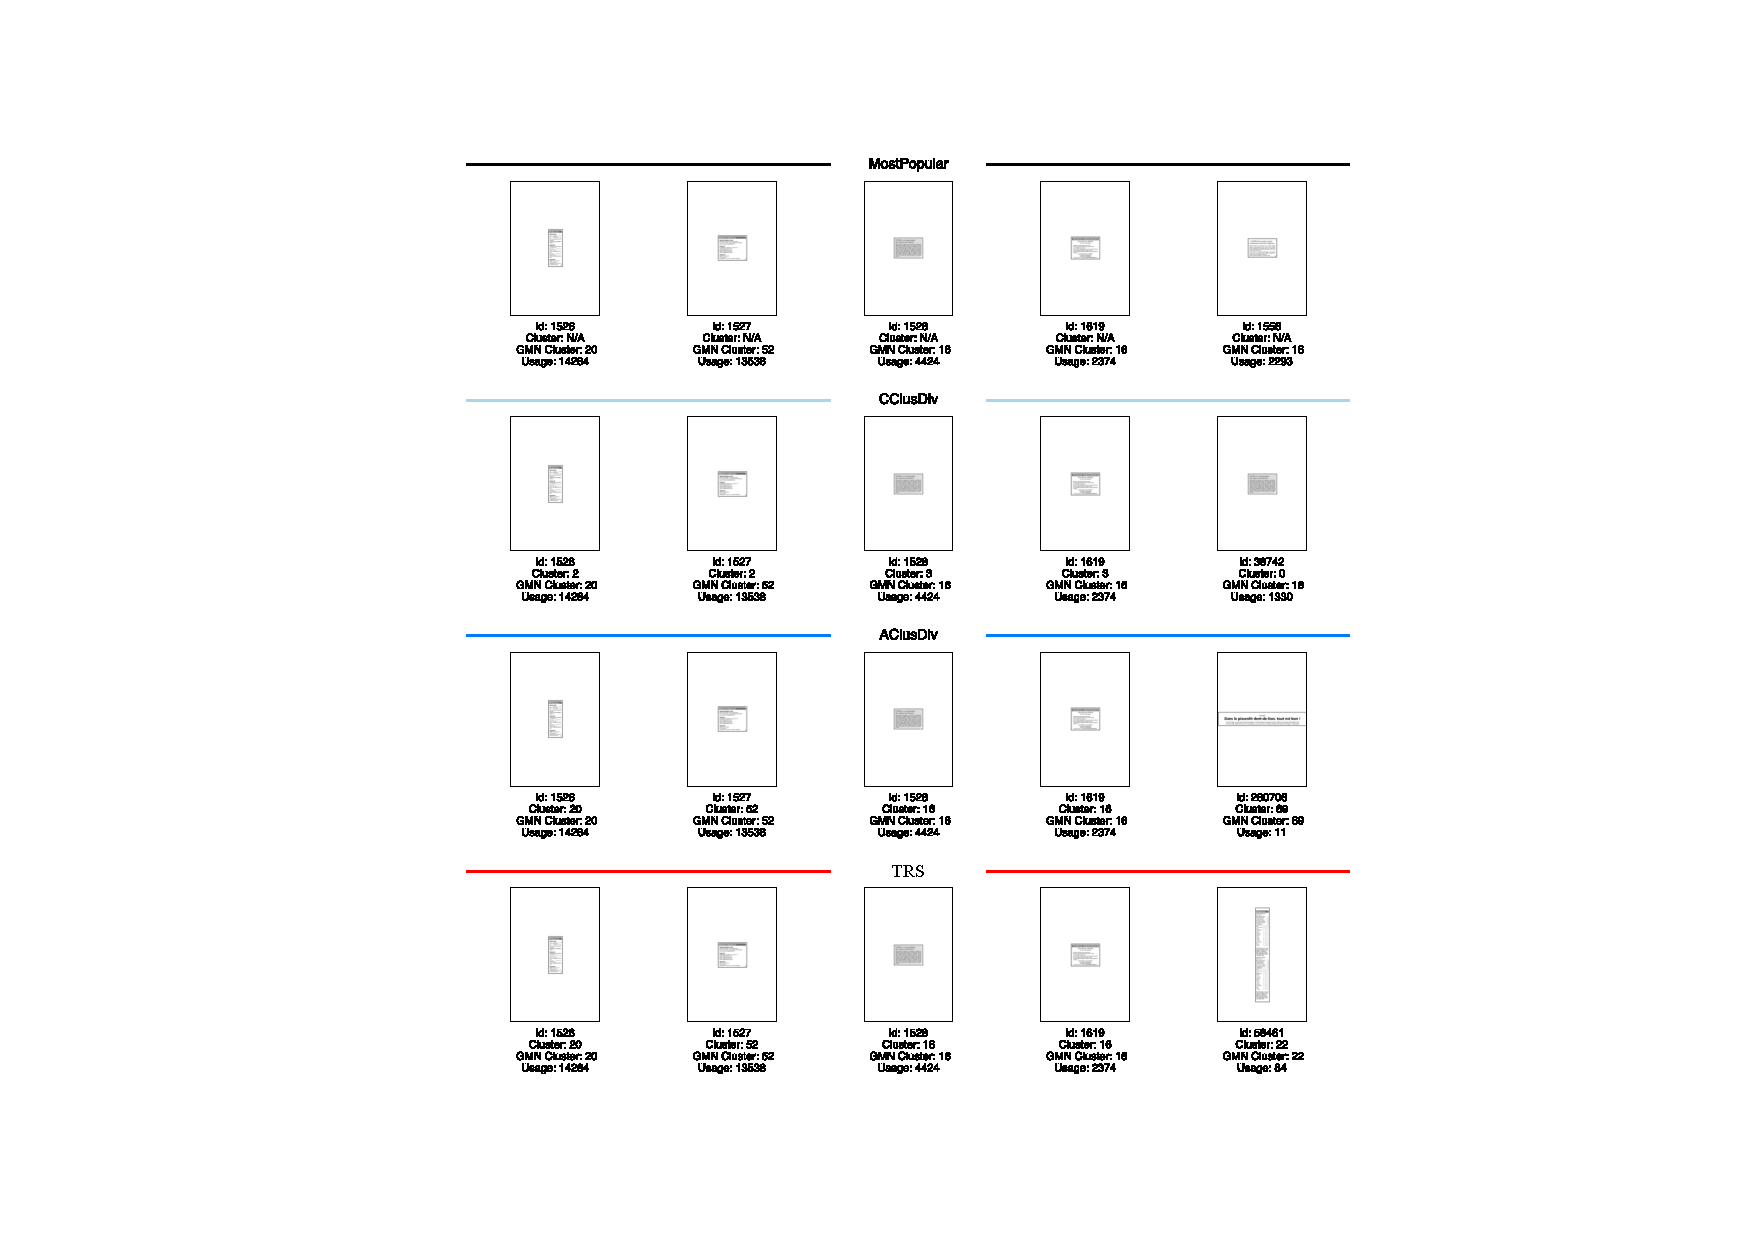
\includegraphics[width=\widthForOneImage]{img/example_prompt_ex_4.pdf}
    \caption{
    Comparison of the top 5 recommended templates with zero images (no title requirement) generated by baseline methods and \trs. IDs, corresponding clusters (if applicable), and usage are reported. Additionally, the GMN-based cluster is indicated for comparison.
    This figure highlights how our method improves diversity not only by similarity-based clustering (like \adaptedclusdiv), but also via our proposed cluster selection during the $CW$-reassignment step. DSTS selects the farthest cluster to break ties between the smallest $CW_i$ values, which promotes templates that are even more distinct from one another.
     }
     \label{fig:example-2} 
\end{figure}

Both examples show that \trs effectively promotes diversity while complying with historical comformity. \classicclusdiv fails to achieve template diversity due to its lack of consideration for structural layout. Although \adaptedclusdiv improves diversity by accounting for layout structure, our approach goes further by leveraging inter-cluster distances and an optimized selection process to maximize structural differences and further enhance diversity.




\section{Page-aware template scoring}
\label{sec:gwes}

In the global page-aware context, template evaluation shifts from isolated single-article selection to assessing candidate template assignments across all articles assigned to a unified page canvas $\page$. This requirement stems from the fact that professional newspaper layouts exhibit tacit structural and visual dependencies, where selecting a template $\templatesel{i}$ for a given article $\articleobj{i}$ inherently depends upon, and influences, the spatial arrangement, aspect ratio, and editorial hierarchy of neighboring articles on the same page canvas.

Evaluating template suitability at the page level requires simultaneously addressing two complementary factors: modeling the internal topological structure of individual templates and capturing the contextual interdependencies among the set of articles $\articleset = \{\articleobj{1}, \articleobj{2}, \dots, \articleobj{n}\}$ co-existing on the page. Standard flat metadata metrics and independent ranking mechanisms are insufficient for this task because they evaluate candidate templates in isolation, failing to capture how spatial configurations interact across adjacent layout blocks to form a cohesive visual spread.

%%%%%% From here keep it
Rather than relying on rigid, handcrafted heuristic rules that fail to capture the nuances of human design, this challenge is addressed by developing a neural evaluation metric that scores the quality of assigned templates $\templatesel{i}$ for each article $\articleobj{i}$ in the page $\page$, considering also their placement in the canvas. This module dynamically scores the contextual harmony between an article's content and its spatial configuration within a newspaper layout, combining a dynamic sequence-level Transformer encoder with a precalculated topological template similarity matrix (using $\gmn{\cdot}{\cdot}$) into a single neural method coined \NeuralMethod\ (\neuralmethod).



\subsection{Problem formulation}
\label{sec:gwes-problem-formulation}

When an article is instead evaluated as part of a page canvas $\page$ shared with other articles $\articleset = \{\articleobj{1}, \dots, \articleobj{n}\}$, editorial harmony between neighboring templates is the goal. 

Formally, the input to this setting is a page canvas $\page$ populated by the article set $\articleset$, each article $\articleobj{i}$ already carrying a candidate template assignment $\templatesel{i}$; this setting is therefore formalized as scoring, rather than retrieving, the compatibility of this joint assignment, conditioned on each article's neighbors on the page. 

Given this formalism, the desired output is a compatibility matrix $\mathbf{P} \in [0,1]^{\numarticles \times \catalogsize}$, where each entry expresses the contextual suitability of assigning a given catalog template to a given article, conditioned on the rest of the page. These per-article scores are later combined with the template similarity matrix $\gmnMatrix$ (\secref{sec:gwes-gmn-mapping}) into a single scalar \neuralmethod\ score for the whole layout $\solution$.

\subsection{Proposed approach}

\neuralmethod\ addresses this problem by combining a Transformer-based encoder, which scores contextual editorial suitability, with the topology-aware similarity metric $\gmn{\cdot}{\cdot}$, which corrects that score for long-tail bias.

\subsubsection{Transformer-based Editorial Intent Module}
\label{sec:transformer_module}

The primary role of the Transformer-based encoder is to operate as a contextual network that scores the appropriateness of each template $\templatesel{i}$ given the specific metadata of each article $\articleobj{i}$ in the set of placed articles $\articleset$ (of size $\numarticles$) and their placement on the page canvas $\page$. Unlike static classification networks, this encoder evaluates the entire page context simultaneously, capturing how the spatial configuration of one article influences the editorial validity of its neighbors.

\paragraph{Input Tensor}

To feed the joint article-template assignment $(\page, \articleset)$ into the Transformer encoder, the article set $\articleset$ (together with each article's currently assigned template $\templatesel{i}$) is reformatted into a single input tensor, aggregating three distinct feature streams per article:
\begin{enumerate}
    \item \textbf{Input Metadata ($\mathbf{m}_i$):} The intrinsic structural features of article $\articleobj{i} \in \articleset$ exactly as defined in Chapter~\ref{chapter:definitions}. This vector encapsulates four concrete numerical features extracted from the input instance: the body text character count, the total number of allocated images, and binary flags indicating the presence of an article title and subtitle, respectively.
    
    \item \textbf{Spatial Coordinates ($\mathbf{c}_i$):} The absolute geometric coordinates of each article $\articleobj{i} \in \articleset$, relative to the page dimensions (\Wpage\ and \Hpage). This vector captures the physical bounding box properties of $\articleobj{i}$, specifically its top-left grid coordinates $(x_i, y_i)$, width $\Wtemp{\templatesel{i}}$, and height $\Htemp{\templatesel{i}}$.
    
    \item \textbf{Template Zoning ($\zoning{i}$):} A flattened structural vector aggregating the internal geometric coordinates of all constituent blocks within template $\templatesel{i}$. For each zoning block $\zblock{i}{k} \in \zoning{i}$, a 5-dimensional feature tuple is appended to the vector, corresponding to a numerical identifier of the semantic feature class $\blockfeat{\zblock{i}{k}}$ (as formalized in Chapter~\ref{chapter:definitions}), followed by its relative bounding box properties $(x, y, w, h)$ normalized by the template dimensions $\Wtemp{\templatesel{i}}$ and $\Htemp{\templatesel{i}}$. This representation captures the layout topology of the template.


\end{enumerate}


For each individual article $\articleobj{i}$, the feature streams are concatenated into a unified vector $\mathbf{x}_i \in \mathbb{R}^{109}$, where the template zoning window is zero-padded up to its maximum  capacity. To evaluate the entire layout as a cohesive unit, the vectors of all $\numarticles$ active articles are sorted from top-to-bottom and left-to-right based on their top-left coordinates, and stacked into a sequence tensor. To accommodate variations in article counts across layouts, these sequences are uniformly padded, while a boolean mask isolates the active articles to evaluate the global page context simultaneously.

\paragraph{Transformer Encoder Model}

The sequence of article vectors $\mathbf{x}_i \in \mathbb{R}^{109}$ representing the layout are subsequently and simultaneously fed into the network. First, a dense linear projection layer maps the 109-dimensional feature space into a 128-dimensional latent embedding space:

\begin{equation}
\mathbf{h}_i^{(0)} = \text{GELU}(\mathbf{W}_p \mathbf{x}_i + \mathbf{b}_p)
\end{equation}
where $\mathbf{W}_p \in \mathbb{R}^{128 \times 109}$ and $\mathbf{b}_p \in \mathbb{R}^{128}$ denote the projection weights and biases, and a Gaussian Error Linear Unit (GELU) activation function introduces non-linear activation thresholds to capture complex editorial compliance patterns. 


To capture the structural hierarchy and sequential sorting order of articles on the page, a learnable positional embedding is additively combined with the projected representations based on each article's sequence index.

This sequence of tokens is subsequently passed to a Transformer encoder~\cite{attention} stack comprised of 4 layers and 8 parallel self-attention heads, with a 512-dimensional feed-forward network. A standard padding mask is applied to restrict the multi-head self-attention mechanism exclusively to the active articles in $\solution$.

Finally, the output of the encoder stack passes through a linear classification softmax layer to generate a probability matrix of dimensions $\numarticles \times \catalogsize$. Each entry in this matrix defines the contextual suitability, expressed as a probability $p\in[0,1]$ of a specific template for a given article in the page layout. 

\subsubsection{tGMN inclusion for template similarity}
\label{sec:gwes-gmn-mapping}

While the Transformer encoder models the dynamic suitability of template assignments based on historical contexts, it is inherently susceptible to long-tail bias, leading to the frequent under-scoring of valid templates simply because they are under-represented in the historical training dataset. This will cause that even if the Transformer achieves high predictive accuracy, its raw probability distributions might be highly concentrated, creating a rigid search space that can cause evolutionary operators to stall. 

To mitigate this, \neuralmethod\ incorporates a precalculated pairwise similarity matrix $\gmnMatrix = [s_{ij}] \in \mathbb{R}^{\catalogsize \times \catalogsize}$ derived from $\gmn{\cdot}{\cdot}$ and $\gmnNetwork$~\cite{patil_layoutgmn_2021, li-gmn-2019}.

However, and because the raw score $\gmn{\cdot}{\cdot}$ is unbounded ($\gmn{\templateobj{i}}{\templateobj{j}} \in (0, \infty], \forall i,j$), these values are mapped into a normalized affinity range $[0,1]$ using a Gaussian kernel transformation:
\begin{equation}
s_{ij} = \exp\left( -\frac{\gmn{\templateobj{i}}{\templateobj{j}}^2}{2(\sigmagmn)^2} \right)
\end{equation}
where $\sigmagmn$ represents a scaling parameter set according to the dataset characteristics to control the smoothness of the topological mapping. This transformation yields the final similarity matrix $\gmnMatrix$, with a bounded similarity score $s_{ij} \in [0, 1]$ between any pair of templates.

\subsubsection{\NeuralMethod (\neuralmethod)}

Finally, to obtain the \neuralmethod, the probabilities from the Transformer and the topological affinities from $\gmnMatrix$ must be algebraically combined. 

Let $\mathbf{P} \in [0,1]^{\numarticles \times \catalogsize}$ be the probability matrix output by the Transformer encoder, where $p_{i,k}$ represents the contextual suitability of assigning template $k$ to article $\articleobj{i}$. Concurrently, let $\templatesel{i} \in \{1, \dots, \catalogsize\}$ denote the  template assignment for said article. The localized compatibility score $\alpha_i$ for article $\articleobj{i}$ is formalized as the dot product between the article's probability distribution and the topological similarity profile of the selected template:
\begin{equation}
\alpha_i = \sum_{k=1}^{\catalogsize} p_{i,k} s_{\templatesel{i}, k}
\end{equation}
where $s_{\templatesel{i}, k}$ is the similarity between the selected template $\templatesel{i}$ and any catalog template $k$, retrieved directly from $\gmnMatrix$. 

This formulation mathematically expresses the probability ``smoothing'' mechanism: if an algorithm or a designer selects a rare template $\templatesel{i}$ that suffers from long-tail bias in the Transformer (yielding a low $p_{i,\templatesel{i}}$), $\alpha_i$ will remain high as long as $\templatesel{i}$ shares a high topological similarity with other frequent templates that received robust probabilities. Finally, to align this metric with a minimization paradigm (necessary for the following chapters), the page-level \NeuralMethod\ (\neuralmethod) score for a layout $\solution$ is aggregated as an editorial mismatch penalty:
\begin{equation}
\neuralmethod(\solution) = \sum_{i=1}^{\numarticles} (1 - \alpha_i)
\end{equation}

\subsection{Experimental evaluation}
\label{sec:gwes-evaluation}

In this section the predictive capabilities and structural behavior of the components underlying the \neuralmethod\ metric are verified. 

\subsubsection{Implementation and Hardware Details}
\label{sec:gwes-implementation}

All deep learning pipelines are powered by the \textit{PyTorch}~\cite{pytorch} ecosystem. This neural framework encompasses the dynamic sequence-level Transformer encoder responsible for predicting historical editorial intent, alongside the implementation of the Layout Graph Matching Network (GMN) utilized to calculate the pre-computed topological affinity matrix~$\gmnMatrix$.

The  training phase for the Transformer Encoder was conducted on a dedicated high-performance GPU computing cluster node, powered by an Intel Xeon Silver 4110 processor, 96~GB of system RAM, and an NVIDIA Tesla T4 GPU with 15~GB of dedicated video memory (VRAM).

\subsubsection{Page Layout and Template Catalog Dataset}

To evaluate the architectural robustness and industrial applicability of the proposed framework, empirical validations were conducted using the available \laprovence archive (\secref{sec:laprovence}). The historical page dataset  provides the required historical context to train the Transformer Encoder module of \neuralmethod. Concurrently, the static template catalog~$\templatecatalog$ serves as the underlying structural dataset utilized to compute the $\gmnMatrix$ matrix.

\paragraph{Historical Layout Dataset}

The historical layout dataset contains a total of $6,007$ production pages extracted from the publisher's workflows. To establish a high-fidelity benchmark, a data-cleaning pipeline was deployed to isolate incomplete or deformed layout files, resulting in $4,449$ fully usable, non-corrupted pages. 

Each layout instance in this clean repository is represented as a detailed XML file encapsulating three data streams:
\begin{itemize}
    \item The global physical dimensions of the page canvas~$\page$, specifying total nominal boundaries ($\Wpage, \Hpage$) and margins ($\mtop, \mbottom, \mleft, \mright$).
    \item The exact top-left coordinate placements ($\xcoord{i}, \ycoord{i}$), dimensions for each individual article~$\articleobj{i}$ relative to the page origin, and the assigned template $\templatesel{i}$.
    \item A structural copy of the internal zoning topology~$\zoning{\templatesel{i}}$, outlining the relative bounding shapes and semantic feature classes of the inner blocks belonging to the chosen template~$\templatesel{i}$.
\end{itemize}

The final dataset consider instances containing a variable count of between $1$ and $11$ distinct news articles arranged simultaneously within a single page canvas.


\paragraph{Template Catalog}

The structural template catalog $\templatecatalog$ is composed by  $\catalogsize = 345$ designs from \laprovence archive. Each blueprint specifies all elements described in Chapter~\ref{chapter:definitions} for a given template: dimensions ($W_j, H_j$), internal zoning $\zoning{j}$ and text capacity mapping $\capacity{j}$. 


\subsubsection{$\gmnMatrix$ calculation}

The structural similarity matrix $\gmnMatrix$ is computed utilizing the template catalog $\templatecatalog$ from \laprovence, but using an instance of $\gmnNetwork$ pre-trained on the analogous, structurally equivalent publishing corpus of \publihebdos, detailed in \secref{section:trs-eval}. 

This calculation outputs a matrix with dimensions $\gmnMatrix = [s_{ij}] \in \mathbb{R}^{345 \times 345}$. Consequently, the training validation and convergence analyses presented in the following sections focus exclusively on the Transformer Encoder architecture. $\gmnMatrix$\  assumes a prominent role  within the evaluation of the unified \neuralmethod\ metric.


\subsubsection{Transformer Encoder Training Hyperparameters}
\label{subsec:hyperparameter_calibration_transformer}

The operational parameters governing the neural training of the Transformer Encoder in \neuralmethod\  were set through extensive empirical pilot studies over the specified dataset. 

The finalized parameters are structured in Table~\ref{tab:algorithmic_parameters_transformer}.

\begin{table}[htbp]
\centering

\begin{tabularx}{\textwidth}{@{}l l X l@{}}
\toprule
Category & Symbol & Parameter Description & Value \\
\midrule
\multirow{7}{*}{\makecell[l]{Transformer \\ Encoder Training}}
           & --- & Neural optimizer architecture & AdamW \\
           & --- & Train/Val/Test split & $80\%/15\%/5\%$ \\
           & --- & Base learning rate & $10^{-4}$ \\
           & --- & Weight decay & $10^{-2}$ \\
           & --- & Batch size & 128 \\
           & --- & Total deep learning training epochs & 3000 \\
           & --- & Early stopping epoch threshold & 40 \\
\bottomrule
\end{tabularx}

\caption{Algorithmic and structural hyperparameters for the Transformer Encoder training.}
\label{tab:algorithmic_parameters_transformer}
\end{table}

\subsubsection{Dataset Split}
The filtered repository of $4,449$ usable pages was passed through a multi-label denoising and stratification pipeline. A global frequency census was executed across all pages to track template occurrences. To ensure that the subsequent split remains mathematically viable for stratified multi-label partitioning, a minimum threshold of three global samples per template class was enforced, guaranteeing adequate representation across the training, validation, and testing folds. Consequently, $67$ pages (representing $1.51\%$ of the corpus) containing orphan or ultra-rare template configurations were removed. 

The remaining $4,382$ production pages were partitioned using an iterative multi-label stratification algorithm with the split ratio indicated in Table~\ref{tab:algorithmic_parameters}. 

\subsubsection{Training Convergence}

The model was trained using cross-entropy loss over a maximum of $3,000$ epochs with an early stopping threshold of $40$ epochs. 

\begin{figure}[htbp]
\centering
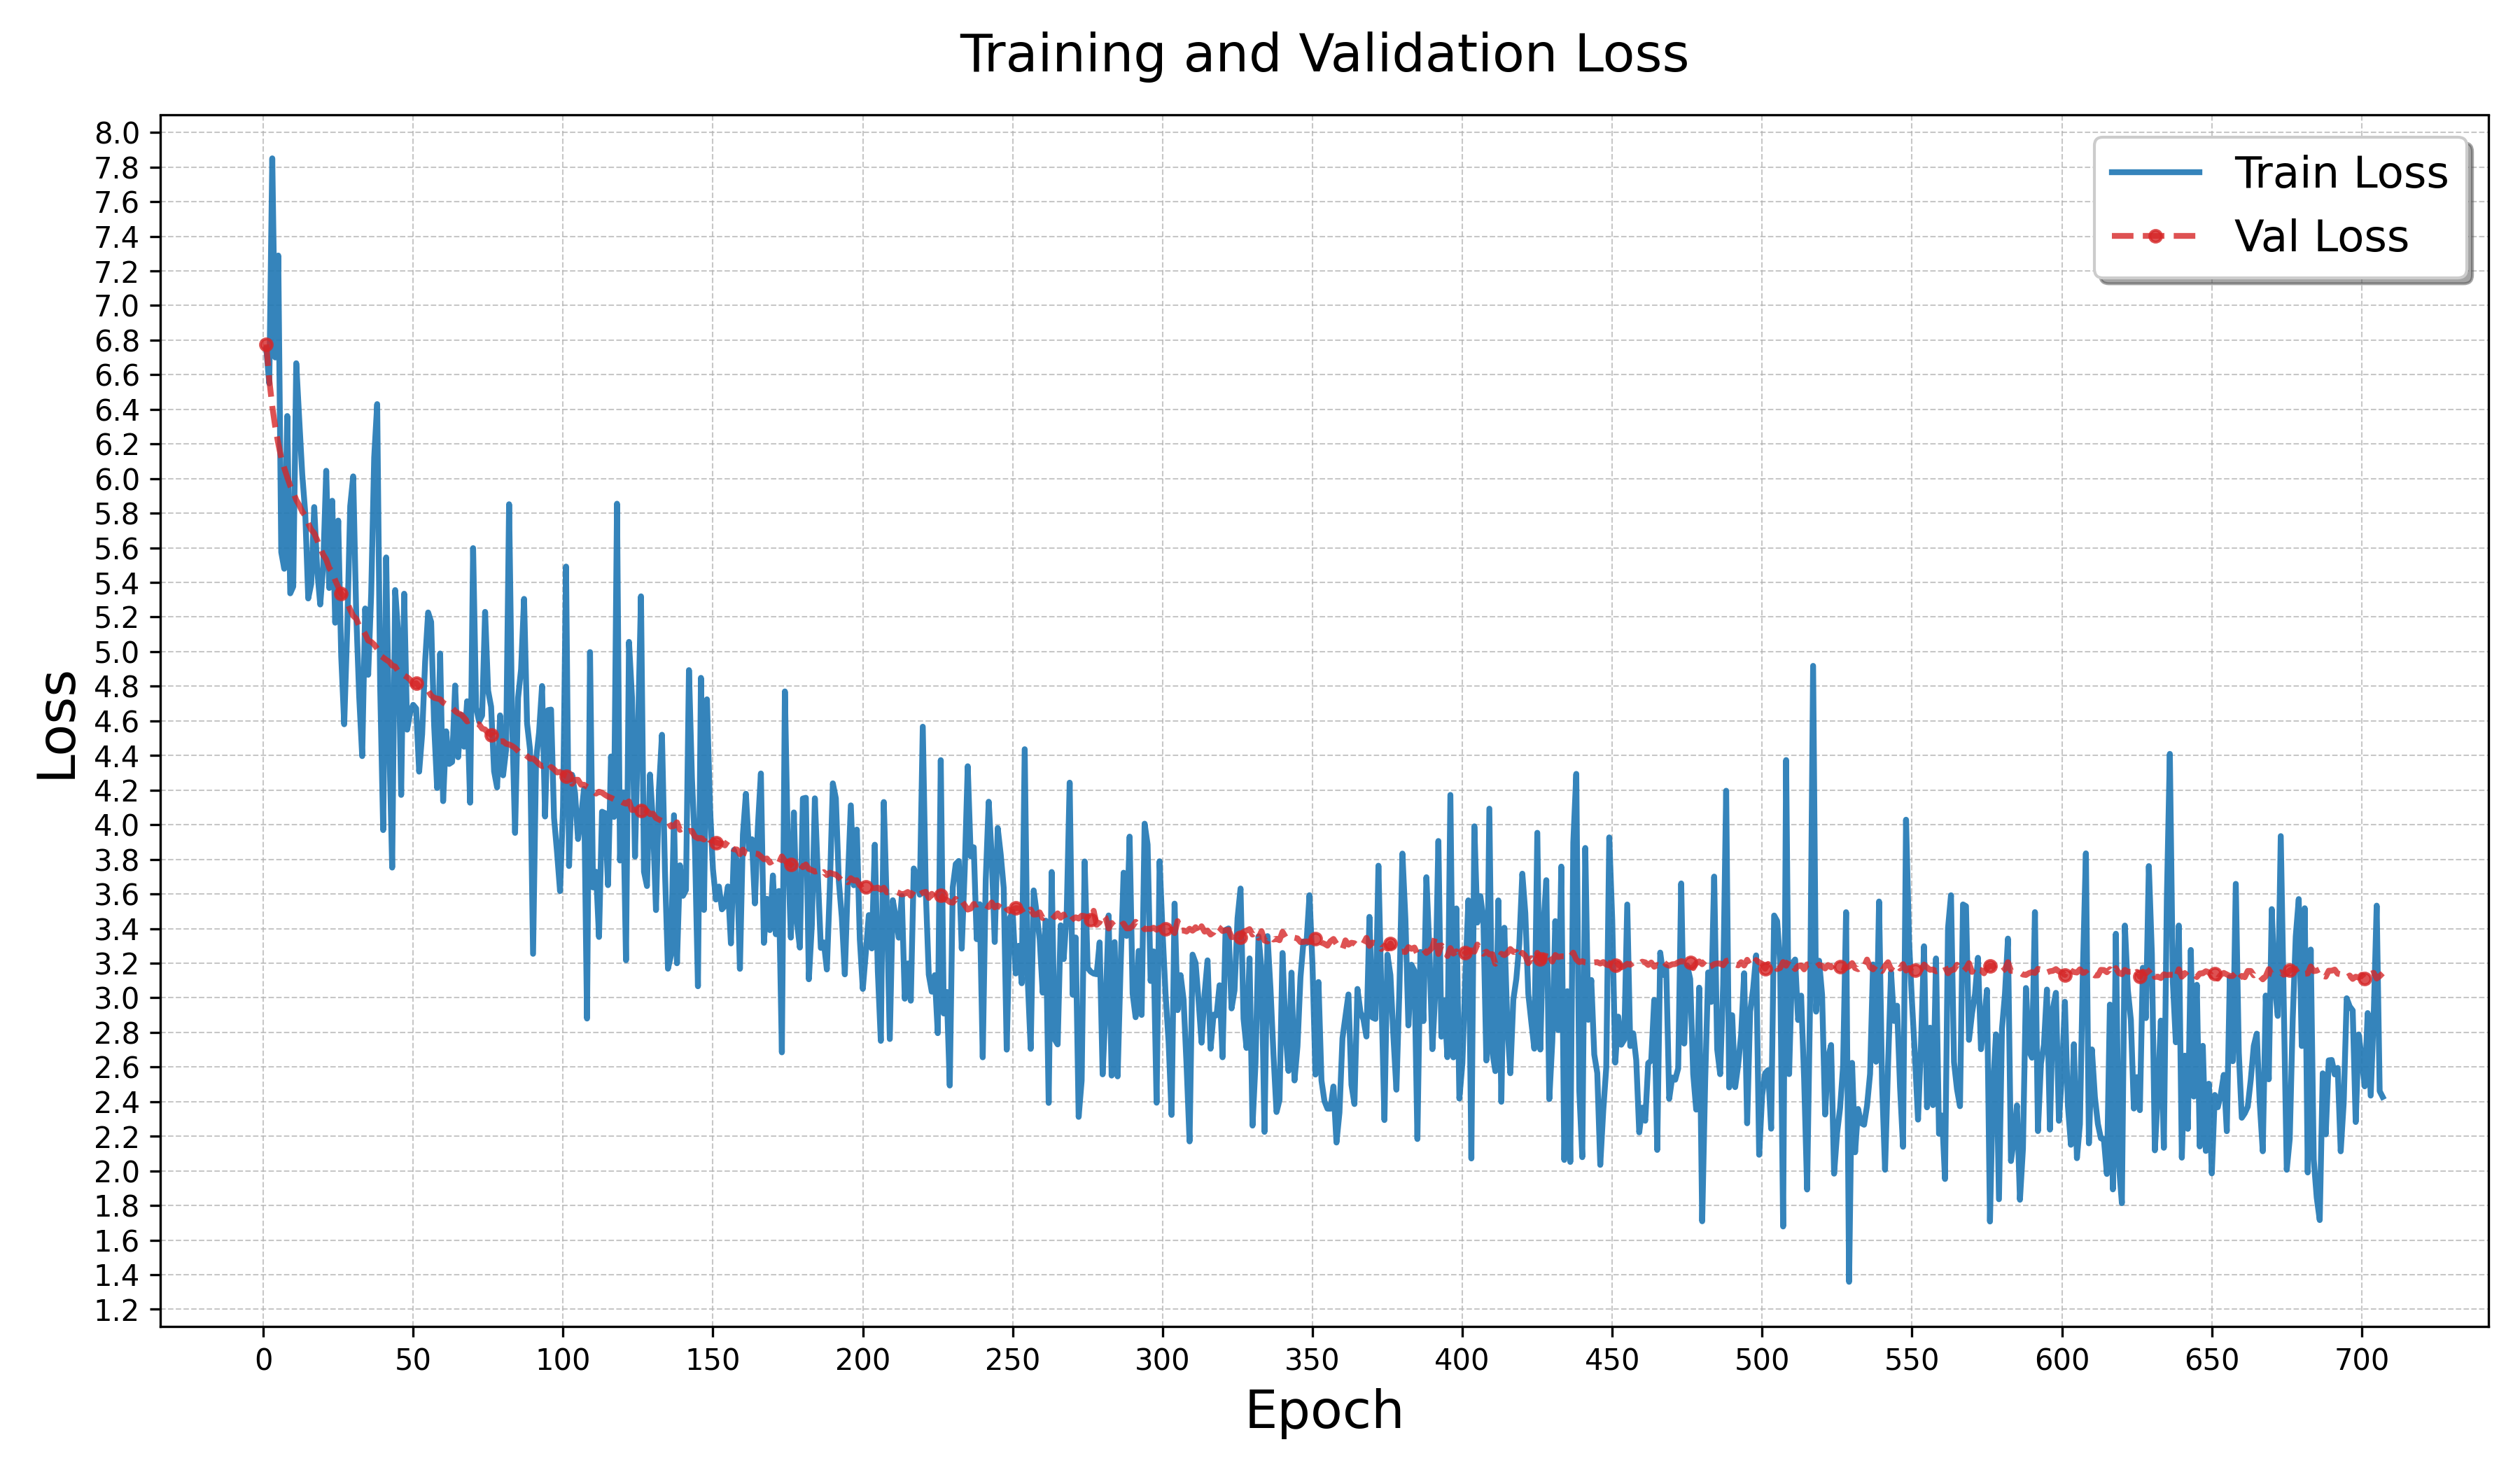
\includegraphics[width=\widthForOneImage]{img/loss_curve.png}
\caption{Training and validation loss curves across optimization epochs.}
\label{fig:loss-curves}
\end{figure}

As illustrated in \figref{fig:loss-curves}, the  oscillations observed in the training loss curve are driven by the intentional feature-dropout protocol applied to the spatial coordinates and zoning matrices during the forward training pass, which introduces controlled batch-level variance. Conversely, during the validation phase, this is not the case and the curve is exceptionally smooth. 

The stabilization of the validation loss at approximately $3.1$ reflects the intrinsic ambiguity of selecting a single exact template from a domain of $\catalogsize = 345$ choices, where multiple configurations can be equally appropriate for the same content. Because cross-entropy heavily penalizes this, the validation loss serves primarily as an internal training convergence guide. Consequently, the true evaluation of the network's performance shifts to the Top-$K$ accuracy rates over the test set and subsequent ablations.


\subsubsection{Predictive Top-K Performance and Feature Ablation}

The dataset split process yielded a definitive test set consisting of $232$ high-fidelity production pages encompassing $587$ individual news articles.

To evaluate both the predictive accuracy and the relative impact of each data stream within the input features, the Top-$K$ accuracy metrics were validated over this independent test set across two operational ablation scenarios: 
\begin{enumerate}
    \item \textit{Metadata Only}: Masking out all absolute coordinates and template zoning details (indices 4--109 reset to $-1.0$) to evaluate predictions based purely on content requirements. This configuration is used when no layout information is available.
    \item \textit{Full Context}: Utilizing the complete information stream, combining raw article metadata, physical coordinates, and internal template zoning topologies.
\end{enumerate}

In all scenarios, a prediction is certified as correct if the target template chosen by the original human designer matches one of the top $K$ highest-probability outputs generated by the softmax distribution. The comparative quantitative results are summarized in Table~\ref{tab:topk_ablation_accuracy}.


\begin{table}[htbp]
    \centering
    \begin{tabularx}{\widthForParametersTable}{Xccc}
    \hline
    \textbf{Available Context} & \textbf{Top-1 Accuracy} & \textbf{Top-3 Accuracy} & \textbf{Top-5 Accuracy} \\ \hline
    Metadata Only & 16.70\% & 35.60\% & 49.23\% \\
    Full Context & 82.62\% & 95.06\% & 97.61\% \\ \hline
    \end{tabularx}
    \caption{Multi-scenario Top-$K$ predictive accuracy and feature ablation rates over the independent test set ($232$ pages, $587$ articles).}
    \label{tab:topk_ablation_accuracy}
\end{table}


The comparative rates in Table~\ref{tab:topk_ablation_accuracy} validate the core assumptions of the hybrid architecture. While the metadata-only scenario exhibits a low Top-1 accuracy of 16.70\% due to the extreme structural ambiguity of predicting a layout without spatial boundaries, its Top-5 accuracy of 49.23\% confirms that the network successfully narrows down the massive search space of 345 designs into a highly relevant subset, providing a good bias for the initialization and mutation operators. Conversely, when the complete physical and zoning context is available, the model achieves an outstanding accuracy, proving that the relational self-attention mechanism successfully captures the latent rules of template assignment.


\subsubsection{$\gmnMatrix$ impact in \neuralmethod}

Although the standalone Transformer Encoder achieves high predictive accuracy, its raw probability distributions are often highly concentrated. To evaluate how the algebraic integration of the LayoutGMN affinity matrix~$\gmnMatrix$ relaxes this constraint boundary without destroying human design alignment, an exhaustive analysis was executed over the test set. 

This validation measures the smoothing effect of the unified \neuralmethod\ metric by capturing flexibility gains across the dataset. For absolute mathematical rigor, because the raw matrix multiplication $\gmnMatrix \cdot \mathbf{V}_{T}^{(i)}$ yields non-normalized structural affinity values, the score vectors were temporarily normalized for the statistical computation to ensure an equivalent probability density domain. This calibration is strictly analytical and restricted to the calculation of these metrics, allowing a fair baseline comparison. The quantitative results of this analysis are summarized in Table~\ref{tab:gmn_impact}.

\begin{table}[htbp]
\centering
\begin{tabularx}{\widthForParametersTable}{Xcc}
\hline
\textbf{} & \textbf{Transformer Only} & \textbf{GWES Resonance}  \\ \hline
Avg. Viable Options ($\text{Prob.} > 5\%$) & 1.89 & 3.23  \\
Max Confidence Peak ($\|\cdot\|_\infty$) & 0.62 & 0.18  \\ \hline
\end{tabularx}
\caption{Quantitative search space relaxation and normalized topological smoothing metrics on the test set ($232$ pages, $587$ articles).}

\label{tab:gmn_impact}
\end{table}

The metrics detailed in Table~\ref{tab:gmn_impact} confirm that the topological convolution step expands the average pool of viable layout alternatives from $1.89$ to $3.23$ options per article, yielding a stable 1.7$\times$ gain in search space flexibility. This phenomenon represents a controlled probability diffusion mechanism, where mass is transferred from isolated predictions toward geometric neighbors. Crucially, this diffusion actively counteracts predictor rigidity, achieving a $71.14\%$ reduction in the distribution's maximum confidence peak (with the mean infinity norm dropping from $0.62$ down to $0.18$). While this smooth distribution naturally lowers the absolute dominance of the top-1 template due to mass sharing among interchangeable designs (while maintaining top-1 rank dominance in general), it successfully transforms a highly polarized search space into a cooperative landscape suitable for optimization tasks.

\begin{figure}[htbp]
\centering
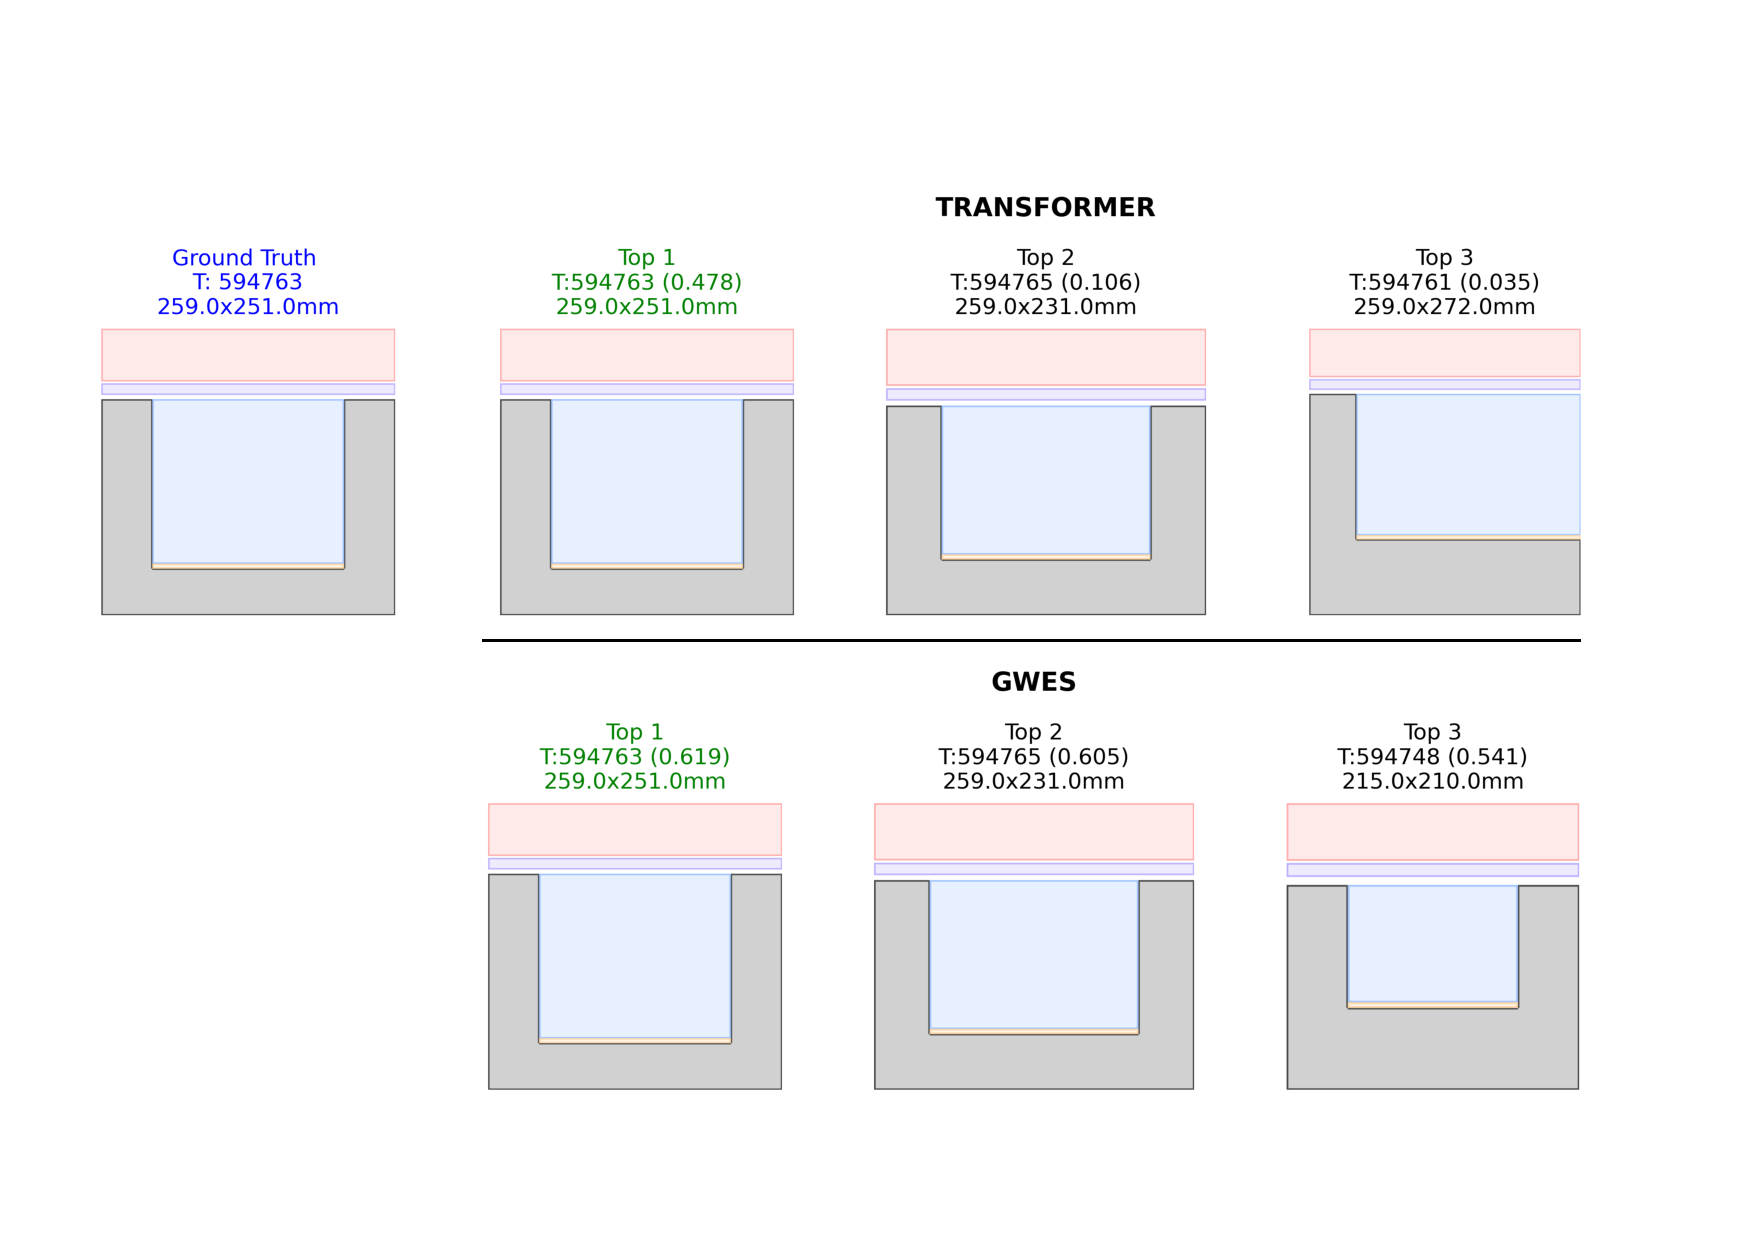
\includegraphics[width=\widthForOneImage]{img/gwes_vs_transformer_ex2.pdf}
\caption{Qualitative behavior of $\gmnMatrix$ smoothing of the Transformer Encoder, for a ground truth target (in blue). Green labels denote the target template. While the raw Transformer pipeline (top row) operates over a formal probability distribution summing to unity, the integrated \neuralmethod\ framework (bottom row) maps raw, non-normalized structural affinity scores derived from the matrix multiplication with $\gmnMatrix$. }
\label{fig:gwes-vs-transformer}
\end{figure}


This behavioral characteristic is qualitatively illustrated in \figref{fig:gwes-vs-transformer}. As shown in this representative example, the human-selected target template (\texttt{T:594763}) is successfully identified as the top rank by both paradigms. However, the standalone Transformer exhibits a rigid, steep probability drop-off immediately after its first choice, collapsing from $0.478$ down to $0.106$ and $0.035$ for the subsequent positions. This polarization penalizes structurally similar alternatives, severely limiting the exploration capacity of the evolutionary engine if the top candidate encounters conflicts.


Conversely, the unified \neuralmethod\ metric leverages the graph-matching prior to build a cooperative, high-utility plateau. To reflect the true operational reality of the evolutionary process, the values displayed for \neuralmethod\ in \figref{fig:gwes-vs-transformer} correspond to the raw, non-normalized affinity scores rather than formal probabilities. Under this framework, \neuralmethod\ actively expands the search space by shifting values; the target template achieves a dominant affinity score of $0.619$, while its direct visual twin (\texttt{T:594765}) is elevated to an equivalent affinity score of $0.605$.







\section{Discussion}
\label{sec:template-discussion}

% TODO(new-prose): discutir trade-offs tdIoU vs. tGMN, TRS vs. GWES, limitaciones.

\section{Conclusion}

% TODO(new-prose): cerrar el capítulo retomando las contribuciones (tdIoU, tGMN, TRS, GWES) y su impacto.



\subsection*{Deployment}

\trs\ was deployed successfully on a pre-production server within \melody's infrastructure, exposed as a Python REST API, and is currently serving as a pilot functionality for the \publihebdos press group~\cite{publihebdos}. This deployment surfaced two a posteriori adaptations, asked directly by this press group:

\begin{itemize}
    \item \textbf{Relaxed image-slot admissibility:} the criterion originally required an exact match between the number of active image slots retained, $\kactive{i} = \Nimg{i}$, and the article's requested image count. In production, a template with more image slots than strictly required by the article is now also considered admissible, provided the article's body text length $\Cart{i}$ falls within the text capacity interval defined by the capacity matrix $\capacity{j}$ (\secref{sec:template}) for some smaller number of active images $k < \Nimgmax{j}$, leaving the remaining slots unused rather than requiring an exact image-count match.
    \item \textbf{Re-ranking presentation instead of a highlighted recommendation:} \publihebdos did not want the recommended templates visually distinguished as an ``intelligent recommendation'' within the production interface. The deployed variant of \trs\ therefore sets $\topsize$ to half the size of the admissible template set and adapts $\cwthreshold$ to the minimum value that still guarantees diversity while allowing exactly $\topsize/2$ templates to be recommended. Under this configuration, the interface simply lists templates in the order returned by \trs, without a dedicated recommendation marked as an AI-driven suggestion.
\end{itemize}

Deployment details specific to \neuralmethod\ (\secref{sec:gwes}) are reported instead in the Deployment section of Chapter~\ref{chapter:pagegen}, since \neuralmethod\ is deployed there as part of \methodNameGeneral.

\subsection*{Publications}

This chapter's contribution on topology-aware template similarity and retrieval is based on the following manuscript, currently under review. The page-aware extension developed in Section~\ref{sec:gwes} (\neuralmethod) is presented here as part of the template retrieval formalism, but is reported instead as a contribution of Chapter~\ref{chapter:pagegen}, whose manuscript is currently in preparation.


\begin{callout}
S. Gallardo, B. G\'enuit, E. Castet, \& P. Kornprobst (2026). \emph{Diversity-Aware Retrieval of Structured Layout Templates via Graph-Matching Network-Based Clustering}. Submitted to \emph{IEEE Access}, under review~\citemine{gallardo-recsys}.
\end{callout}


